\chapter {DASAR TEORI}

Pada bab ini, akan dijelaskan dasar teori yang digunakan sebagai landasan pengerjaan tugas akhir ini akan dijabarkan. Pertama, bab ini akan menjelaskan mengenai deskripsi soal \textit{Factorial Modulo Prime}. Kemudian, pembahasan mengenai analisis soal beserta dengan beberapa metode penyelesaian yang dapat digunakan akan dijabarkan.

\section{Deskripsi Permasalahan}
Permasalahan yang akan dibahas pada tugas akhir ini adalah komputasi nilai dari $ N! $ dalam modulo $ P $, dimana $ P $ adalah bilangan prima. Faktorial didefinisikan pada persamaan \eqref{eq:persamaan_faktorial}.
\begin{equation}
	N! = \prod_{i=1}^{N} i
	\label{eq:persamaan_faktorial}
\end{equation}
Besarnya batasan pada permasalahan ini adalah $ 0 \leq N \leq 10^{11} $, $ P = \{\ p\ |\ 2 \leq p \leq 10^{11} , p \in prima \} $ dengan batas waktu $ 10-15 $ detik untuk setiap file uji yang diberikan. Komputasi $ N! $ dalam modulo $ P $ pada umumnya memiliki kompleksitas $ \mathcal{O}{(N)} $, sehingga akan melebihi batas waktu yang diberikan.

Penulis menemukan terdapat dua algoritma yang bisa diadaptasikan untuk menyelesaikan permasalahan komputasi ini yaitu \textit{Multipoint Evaluation} dan \textit{Shifting Evaluation Values}.

\section{Deskripsi Umum}

Subbab ini akan memaparkan definisi, deskripsi dan landasan yang akan digunakan pada keseluruhan penyelesaian masalah.

\subsection{Modulo}
Didalam matematika, modulo adalah sebuah operasi yang menghasilkan sisa pembagian (\textit{remainder}) dari suatu bilangan terhadap bilangan lainnya. Operasi pembagian bilangan $ a $ dengan $ b $ pada dasarnya merupakan bentuk lanjut dari persamaan \eqref{eq:persamaan_umum_pembagian}
\begin{equation}
	\begin{aligned}
		b \in \mathbb {Z}\\
		a=qb+r\\
		0 \leq r < b \\
	\end{aligned}
	\label{eq:persamaan_umum_pembagian}
\end{equation}

Nilai $ q $ pada persamaan \eqref{eq:persamaan_umum_pembagian} disebut dengan \textit{quotient}, merupakan hasil bagi dari $ \frac{a}{b} $, sedangkan nilai $ r $ pada persamaan \eqref{eq:persamaan_umum_pembagian} disebut dengan \textit{remainder} atau \textit{modulus} yang merupakan sisa hasil bagi. Operasi modulo sering digunakan untuk menghindari \textit{integer overflow} karena dipastikan hasil operasi modulo berada didalam rentang $ [0,b) $.

Modulo memiliki kaitan erat dengan kongruensi, kongruensi adalah kesamaan nilai \textit{remainder} atau \textit{modulus} dua bilangan terhadap sebuah nilai pembagi. Dengan kata lain, dua bilangan $ a $ dan $ b $, memiliki kongruensi (atau cukup disebut kongruen) terhadap sebuah nilai $ n $ apabila $a \Mod{n}=b \Mod{n}$. Notasi yang umum digunakan untuk menggambarkan kongruensi dapat dilihat pada persamaan \eqref{eq:kongruensi}.
\begin{equation}
	a\equiv b \Mod{n}
	\label{eq:kongruensi}
\end{equation}

Kongruensi memiliki beberapa sifat.\cite{stallings_cryptography}
\begin{enumerate}
	\item $ a\equiv b \Mod{n} $ apabila $ n|(a - b) $, yaitu $ n $ habis membagi $ a-b $.
	\item Kongruensi bersifat komutatif. Yaitu $ a\equiv b \Mod{n} $ mengindikasikan bahwa $ b\equiv a \Mod{n} $.
	\item Kongruensi bersifat transitif. Yaitu $ a\equiv b \Mod{n} $ dan $ b\equiv c \Mod{n} $ mengindikasikan bahwa $a \equiv c \Mod{n} $.
\end{enumerate}

\subsection{Aritmatika Modular}
Sistem kongruensi dapat dioperasikan menggunakan operasi matematika pada umumnya \cite{stallings_cryptography}, yang selanjutnya disebut aritmatika modular.

\subsubsection{Operasi Dasar}
Operasi dasar yang dapat dioperasikan pada sistem kongruensi yaitu penjumlahan, pengurangan, perkalian, dan pembagian.

\begin{enumerate}
\item Penjumlahan \\
	Diberikan dua nilai $ a $ dan $ b $ serta modulo $ n $, maka 
	\begin{equation}
		a\ \Mod{n}+b\ \Mod{n}\equiv a+b\ \Mod{n}
		\label {eq:mod_jumlah}
	\end{equation}

	Persamaan \eqref{eq:mod_jumlah} dapat ditulis sebagai persamaan \eqref{eq:mod_jumlah_long}.
	\begin{equation}
		[a\ \Mod{n}+b\ \Mod{n}]\ \Mod{n}\equiv a+b\ \Mod{n}
		\label {eq:mod_jumlah_long}
	\end{equation}

\item Pengurangan \\
	Diberikan dua nilai $ a $ dan $ b $ serta modulo $ n $, maka 
	\begin{equation}
		a\ \Mod{n}-b\ \Mod{n}\equiv a-b\ \Mod{n}
		\label{eq:mod_kurang}
	\end{equation}

	Persamaan \eqref{eq:mod_kurang} dapat ditulis sebagai persamaan \eqref{eq:mod_kurang_long}.
	\begin{equation}
		[a\ \Mod{n}-b\ \Mod{n}]\ \Mod{n}\equiv a-b\ \Mod{n}
		\label {eq:mod_kurang_long}
	\end{equation}

\item Perkalian \\
	Diberikan dua nilai $ a $ dan $ b $ serta modulo $ n $, maka 
	\begin{equation}
		a\ \Mod{n}*b\ \Mod{n}\equiv a*b\ \Mod{n}
		\label{eq:mod_kali}
	\end{equation}

	Persamaan \eqref{eq:mod_kali} dapat ditulis sebagai persamaan \eqref{eq:mod_kali_long}.
	\begin{equation}
		[a\ \Mod{n}*b\ \Mod{n}]\ \Mod{n}\equiv a*b\ \Mod{n}
		\label{eq:mod_kali_long}
	\end{equation}

\item Pembagian \\
	Diberikan dua nilai $ a $ dan $ b $ serta modulo $ n $, maka 
	\begin{equation}
		a\ \Mod{n}* b^{-1}\ \Mod{n}\equiv a*b^{-1}\ \Mod{n}
		\label{eq:mod_bagi}
	\end{equation}

	Persamaan \eqref{eq:mod_bagi} dapat ditulis sebagai persamaan \eqref{eq:mod_bagi_long}.
	\begin{equation}
		[a\ \Mod{n}*b^{-1}\ \Mod{n}]\ \Mod{n}\equiv a*b^{-1}\ \Mod{n}
		\label{eq:mod_bagi_long}
	\end{equation}

	Operasi pembagian memerlukan nilai dari \textit{inverse modulus} dari $ b $ yang dilambangkan $ b^{-1}\ \Mod{n} $, dimana harus memenuhi persamaan \eqref{eq:mod_kali_invers}

	\begin{equation}
		b \cdot b^{-1} \equiv 1 \Mod{n}
		\label{eq:mod_kali_invers}
	\end{equation}

\end{enumerate}

\subsubsection{Modulo Inverse}
Untuk menghitung nilai modulo inverse dari $ b $ dalam modulo $ n $, dimana $ n $ disini merupakan bilangan prima, mengacu pada soal \nomorsoal\ \soal, sehingga bisa menggunakan Teorema \ref{theo:fermat_little_theorem}, untuk membantu menyelesaikan pencarian modulo inverse.

\begin{theo}[Fermat's Little Theorem]
	\label{theo:fermat_little_theorem}
	Jika $ P $ adalah sebuah bilangan prima, maka untuk sembarang integer $ a $, $ a^p - a $ adalah kelipatan dari $ P $.
	\begin{equation}
		\begin{aligned}
			a^{P} \equiv a \Mod{P} \\
			a^{P-1} \equiv 1 \Mod{P} \\
		\end{aligned}
		\label{eq:fermat_theorem}
	\end{equation}
\end{theo}
Menggunakan persamaan \eqref{eq:fermat_theorem}, dan membagi kedua sisi dengan $ a $ maka didapatkan persamaan \eqref{eq:modulo_inverse}.
$$ \frac{a^{P-1}}{a} \equiv \frac{1}{a} \Mod{P} \\ $$
\begin{equation}
	a^{P-2} \equiv a^{-1} \Mod{P} \\
	\label{eq:modulo_inverse}
\end{equation}
Sehingga modulo inverse dari $ b $ kongruen dengan $ b^{n-2} $ dalam modulo $ n $, dimana $ n $ merupakan bilangan prima.

\subsection{Perpangkatan Modular}
Operasi perpangkatan diperlukan dalam perhitungan modulo inverse dari $ b $ dalam modulo $ n $, dengan menggunakan properti persamaan \eqref{eq:mod_kali_long} dapat dilakukan perpangkatan secara \textit{na\"ive}. Tetapi jika mempertimbangkan efisiensi dalam perpangkatan, misal untuk menghitung $ a^n $, solusi \textit{na\"ive} memerlukan kompleksitas $ \mathcal{O}{(n)} $.
$$ a^n = a \cdot a \cdots a\ (n\ kali) $$

Namun, hasil yang sama bisa diperoleh dengan kompleksitas lebih rendah, jika menggunakan metode \textit{fast modular exponentiation}, yaitu mengubah bilangan pemangkat yaitu $ n $ menjadi basis biner terlebih dahulu, lalu dilakukan perkalian bertahap, untuk contoh dalam menghitung nilai dari $ x^{11} $
$$ x^{11} = x^{1+2+8} = (x)(x^{2})(x^{8}) $$
atau dalam kongruensi 
$$ x^{11}\ \mod{n} \equiv [(x\mod{n})(x^{2}\mod{n})(x^{8}\mod{n})]\mod{n} $$

Secara general, menghitung nilai dari $ a^b\mod{n} $, dengan $ a $ dan $ b $ adalah bilangan bulat, maka kita bisa mengubah $ b $ dalam basis biner $b_{k} b_{k-1} b_{k-2} \cdots b_{0}$, seperti persamaan \eqref{eq:basis_biner_b}.

\begin{equation}
	b = \sum_{b_i \neq 0} 2^i
	\label{eq:basis_biner_b}
\end{equation}

Kemudian, dengan mensubstitusikan $ b $ dari persamaan \eqref{eq:basis_biner_b}, didapatkan persamaan \eqref{eq:modular_expo}.

$$ a^b = a^{\sum_{b_i \neq 0} 2^i} = \prod_{b_i \neq 0} a^{2^{i}} $$
\begin{equation}
	a^b\mod{n} = \left [ \prod_{b_i \neq 0} a^{2^{i}} \mod{n} \right ] \mod{n}
	\label{eq:modular_expo}
\end{equation}

Dalam menghitung nilai dari $ a^{2^{i}} $, dapat dilakukan secara iteratif, sehingga persamaan \eqref{eq:modular_expo} dapat ditulis kembali menjadi persamaan \eqref{eq:modular_expo_f_y}.

\begin{equation}
	\begin{aligned}
	a^b\mod{n} = \left [ \prod_{k = 1} f_y(k)\right ] \mod{n} \\
	f_y(k)=
		\begin{cases}
			1,  					& \text{if } b_k=0 \\
			a^{2^{k}}  \mod{n} ,   & \text{if } b_k=1
		\end{cases} \\
	\end{aligned}
	\label{eq:modular_expo_f_y}
\end{equation}


Dengan persamaan \eqref{eq:modular_expo_f_y} dapat dibuktikan perhitungan $ a^b \mod{n} $ membutuhkan $ log_2\ b $ perkalian, sehingga \textit{fast modular exponentiation} atau perpangkatan modular \textit{repeated squaring} memiliki kompleksitas $ \mathcal{O}{(log_2\ n)} $. 

Bedasarkan penjelasan diatas bisa disusun pseudocode \textit{fast modular exponentiation} yang ditunjukkan oleh pseudocode \ref{psdo:fast_modex}.

\begin{algorithm}
	\caption{Fast Modular Exponentiation}
	\label{psdo:fast_modex}
	\begin{algorithmic}[1]
		\Require $a,\ b,\ n$
		\Ensure $y = a^b\mod{n}$
		\State $y \leftarrow 1$
		\While{ $ b > 0 $}
			\If {$ b $\ is\ odd}
				\State $ y = y \cdot a $
			\EndIf
			\State $ b = b / 2 $
			\State $ a = a \cdot a $
		\EndWhile \\
		\Return $ y $
	\end{algorithmic}
\end{algorithm}

Pada subbab berikutnya akan dibahas metode efisien dalam perkalian modular, serta implementasi dalam operasi aritmatika modular lainnya.

\subsection{Perkalian Modular Montgomery}
Perkalian Modular \textit{Montgomery} atau reduksi \textit{montgomery} adalah metode efisien untuk menghitung $ u = a \cdot b \Mod{n} $ dengan $ a, b, $ dan $ n $ adalah  bilangan $k$-bit, yang dikenalkan oleh Peter L. Montgomery pada tahun 1985 \cite{montgomery}. 

Algoritma ini cocok digunakan dalam implementasi pada software dan hardware komputer karena kemampuannya dalam melakukan operasi modulo pangkat 2 dengan cepat. Reduksi untuk menghasilkan $ u $ tidak dilakukan dengan cara pembagian dengan $ n $ seperti pada perkalian modulo pada umumnya, tetapi dengan $ 2^r $ dalam representasi \textit{Montgomery World}.

Asumsikan modulus $ n $ adalah bilangan $k$-bit sedemikian hingga $ 2^{k-1} \leq n < 2^{k} $ dan $ r = 2^{k}$. Perkalian modular \textit{montgomery} memerlukan nilai $ r $ dan $ n $ yang relatif prima sedemikian hingga $ gcd(r, n) = gcd(2^k, n) = 1 $. Persamaan diatas dapat dipenuhi apabila $ n $ adalah bilangan ganjil.

Diberikan bilangan bulat $ a < n $ dan $ b < n $, yang dalam representasi \textit{Montgomery World} dengan $ r $ dilambangkan dalam persamaan \eqref{eq:mont_world}
\begin{equation}
	\begin{aligned}
		\bar{a} = a \cdot r \Mod{n} \\
		\bar{b} = b \cdot r \Mod{n} \\
	\end{aligned}
	\label{eq:mont_world}
\end{equation}
Perkalian modular \textit{montgomery} didefinisikan dalam persamaan \eqref{eq:mont_mul}
\begin{equation}
	x = \bar{a} \cdot \bar{b} \cdot r^{-1} \Mod{n}
	\label{eq:mont_mul}
\end{equation}
$ r^{-1} $ adalah modulo inverse dari $ r $ dalam modulo $ n $. Langkah selanjutnya adalah reduksi, dalam reduksi \textit{montgomery} memperlukan nilai dari $ n' $ yang bisa didapatkan melalui property \eqref{eq:mont_property}
\begin{equation}
	r \cdot r^{-1} - n \cdot n' = 1
	\label{eq:mont_property}
\end{equation}
sehingga nilai $ n' $ dilambangkan persamaan \eqref{eq:mont_n_aksen}
\begin{equation}
	n' = \frac{r(r^{-1}\mod{n}) -1}{n}
	\label{eq:mont_n_aksen}
\end{equation}

Perkalian modular \textit{montgomery} lebih cocok digunakan dalam \textit{chain multiplication} dengan modulo tetap, sehingga algoritma ini dapat digunakan dalam pseudocode \ref{psdo:fast_modex}.Algoritma perkalian modular \textit{montgomery} dapat dirangkum dalam pseudocode \ref{psdo:montgomery}. 

\begin{algorithm}
	\caption{Perkalian Modular Montgomery}
	\label{psdo:montgomery}
	\begin{algorithmic}[1]
		\Require $a,\ b,\ n$
		\Ensure $c = ab\mod{n}$
		\State $r = 2^n $, $ r \in \mathbb{N}, r > n, gcd(r,n) = 1 $
		\State $n' = \frac{r(r^{-1}\mod{n}) -1}{n} $
		\State $\bar{a} = a \cdot r \Mod{n} $
		\State $\bar{b} = b \cdot r \Mod{n} $
		\State $x = \bar{a}\bar{b} $
		\State $s = (x \cdot n'\ \mod{r}) $
		\State $t = x + sn $
		\State $u = \frac{t}{r} $
		\If{$u < n$}
			$\ \bar{c} = u $
		\Else
			$\ \bar{c} = u - n $
		\EndIf \\
		\Return $ c = \bar{c}r^{-1}\mod{n} $.
	\end{algorithmic}
\end{algorithm}

Selain perkalian, \textit{montgomery} bisa diterapkan untuk operasi seperti pertambahan dan pengurangan, karena sifat distribusi yang dimiliki modulo.
$$ ar + bR = (a+b)r $$
$$ ar - bR = (a-b)r $$
Sementara untuk operasi pembagian, hampir sama dengan pembagian modular biasa, dengan mengalikan dalam \textit{Montgomery World} dengan inversenya.
$$ \frac{a}{b}r = ar \cdot b^{-1}r $$

\subsection{Fast Fourier Transform}
Pada tahun 1965, James W. Cooley dan John W. Tukey berhasil merumuskan suatu teknik perhitungan algoritma \textit{Fourier Transform} yang efisien\cite{fft}. Teknik perhitungan algoritma ini dikenal dengan sebutan \textit{Fast Fourier Transform} atau lebih populer dengan istilah FFT. \textit{Fast Fourier Transform} dalam bahasa indonesia adalah Transformasi Fourier Cepat adalah sumber dari suatu algoritma untuk menghitung \textit{Discrete Fourier Transform (DFT)} atau Transformasi Fourier Diskrit dengan cepat dan efisien beserta dengan inversenya.

Transformasi Fourier Cepat diterapkan dalam berbagai bidang mulai dari pengolahan signal digital, memecahkan persamaan differensial parsial, sampai dalam perkalian polinomial. Ada pun kelas dasar dari algoritma FFT yaitu \textit{Decimation in Time (DIT)} dan \textit{Decimation in Frequency (DIF)}. Pada subbab ini akan dijelaskan FFT yang digunakan untuk perkalian polinomial dengan \textit{Decimation in Time (DIT)}.

Ide yang digunakan FFT dalam perkalian polinomial adalah, jika ingin mengkomputasi perkalian polinomial $ fg $, evaluasi polinomial $ f(x) $ dan $ g(x) $ pada banyak titik $ x_m $, kemudian mengalikan $ f(x_m) \cdot g(x_m) $, kemudian mencari polinomial yang melalui titik titik tersebut. Mungkin pencarian polinomial dari beberapa titik bisa menggunakan metode standar yaitu interpolasi langrange, tetapi dikarenakan kompleksitas yang besar, kita perlu memikirkan jalan lain.

Disinilah Transformasi Fourier Diskrit berperan, jika kita ingin mengalikan 2 polinomial dengan derajat maksimal 7, maka diperlukan 8 nilai dari $ x_m $, sehingga kita memerlukan 8\textit{-th roots of unity}.
$$ \omega_8 = \exp(\frac{-2\pi i}{8}) , x_m = \omega^m, 0 \leq m \leq 7 $$
\textit{Roots of unity} adalah $ n $ bilangan kompleks yang memenuhi $ z^{n} = 1 $. Untuk transformasi fourier nilai $ \omega_N = \exp(\frac{-2\pi i}{N}) $ dimana $ \omega_N $ merupakan $ N^{th} $ \textit{roots of unity}. Pencarian nilai $ \omega_N $ dapat diselesaikan menggunakan persamaan trigonometri \eqref{eq:trigo_root_of_unity}.
\begin{equation}
	\omega_N = \exp(\frac{2\pi i}{N}) = \cos(\frac{2\pi}{N}) + i \sin(\frac{2\pi}{N})
	\label{eq:trigo_root_of_unity}
\end{equation}
\textit{Roots of unity} akan menjadi pilihan titik-titik yang dijadikan dasar pada evaluasi polinomial. \textit{Roots of unity} juga memiliki properti khusus seperti pada persamaan \eqref{eq:property_root_of_unity}.
\begin{equation}
	\begin{aligned}
		\omega_{N}^{N} = 1 \\
		\omega_{N}^{N+k} = \omega_{N}^{k} \\
		\omega_{N}^{N/2} = -1 \\
		\omega_{N}^{N/2+k} = -\omega_{N}^{k} \\
	\end{aligned}
	\label{eq:property_root_of_unity}
\end{equation}

Dengan menggunakan persamaan \eqref{eq:property_root_of_unity}, polinomial $ f $ dapat di evaluasi, dengan $ f(x) = a_0 + a_1x + .... a_7x^7 $, 
\begin{equation}
	\begin{aligned}
		f(\omega^0) = a_0 + a_1 \ \ \   + a_2\ \ \ \ \ + a_3\ \ \ \ \ + a_4\ \ \ \ \ + a_5\ \ \ \ \ + a_6\ \ \ \ \ + a_7  \ \ \ \ \\ 
		f(\omega^1) = a_0 + a_1\omega^1 + a_2\omega^2 + a_3\omega^3 + a_4\omega^4 + a_5\omega^5 + a_6\omega^6 + a_7\omega^7 \\ 
		f(\omega^2) = a_0 + a_1\omega^2 + a_2\omega^4 + a_3\omega^6 + a_4\ \ \ \ \ + a_5\omega^2 + a_6\omega^4 + a_7\omega^6 \\ 
		f(\omega^3) = a_0 + a_1\omega^3 + a_2\omega^6 + a_3\omega^1 + a_4\omega^4 + a_5\omega^7 + a_6\omega^2 + a_7\omega^5 \\ 
		f(\omega^4) = a_0 + a_1\omega^4 + a_2\ \ \ \  + a_3\omega^4 + a_4\ \ \ \  + a_5\omega^4 + a_6\ \ \ \ \ + a_7\omega^4 \\ 
		f(\omega^5) = a_0 + a_1\omega^5 + a_2\omega^2 + a_3\omega^7 + a_4\omega^4 + a_5\omega^1 + a_6\omega^6 + a_7\omega^3 \\ 
		f(\omega^6) = a_0 + a_1\omega^6 + a_2\omega^4 + a_3\omega^2 + a_4\ \ \ \ \ + a_5\omega^6 + a_6\omega^4 + a_7\omega^2 \\ 
		f(\omega^7) = a_0 + a_1\omega^7 + a_2\omega^6 + a_3\omega^5 + a_4\omega^4 + a_5\omega^3 + a_6\omega^2 + a_7\omega^1 \\ 
	\end{aligned}
	\label{eq:evaluasi_fft}
\end{equation}

Setelah itu, langkah selanjutnya dalam FFT adalah mengumpulkan menjadi blok-blok tertentu, pengelompokan ini sebenarnya memiliki beberapa metode, seperti pengelompokan ganjil-genap maupun pengelompokan dengan \textit{bit-reverse-index}. Pada contoh ini, penulis menggunakan pengelompokkan ganjil-genap. Apabila index ganjil dan genap dikelompokkan seperti pada gambar \ref{fig:fft_ordering}.
\begin{figure}
	\Centering
	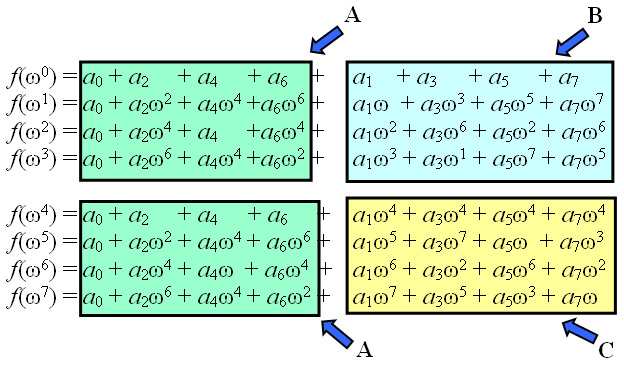
\includegraphics [scale=0.5]{bab2/img/fft_ordering}
	\caption {Pengelompokan Blok FFT}
	\label {fig:fft_ordering}
\end{figure}
Blok berlabel $'A'$ merupakan Transformasi Fourier Diskrit dari $ f(x) = a_0 + a_2x + a_4x^2 + a_6x^3 $, Kemudian block berlabel $'B'$ adalah Transformasi Fourier Diskrit dari $ f(x) = a_1 + a_3x + a_5x^2 + a_7x^3 $ dengan suku ke-$j$ dikalikan dengan $\omega^j$, dengan $j = 0,1,2,3 $. Terakhir block berlabel $'C'$ adalah block dengan negative value dari $'B'$. Kemudian dilakkan secara rekursif pada masing masing DFT baru.

Menggunakan properti pada persamaan \eqref{eq:property_root_of_unity}, maka secara formal pengelompokan bisa diubah menjadi persamaan \eqref{eq:fft_ordering_rumus}
\begin{equation}
	X_k = \sum_{n=0}^{\frac{N}{2}-1} x_{2n}\omega_{\frac{N}{2}}^{kn} + \sum_{n=0}^{\frac{N}{2}-1} x_{2n+1}\omega_{\frac{N}{2}}^{kn}
	\label{eq:fft_ordering_rumus}
\end{equation}
Apabila kita misalkan $ y_n = x_{2n} $ dan $ x_n = x_{2n+1} $ maka didapatkan hasil pada persamaan \eqref{eq:fft-kiri} dan \eqref{eq:fft-kanan}
\begin{equation}
	Y_k = \sum_{n=0}^{\frac{N}{2}-1} y_{n}\omega_{\frac{N}{2}}^{kn}
	\label{eq:fft-kiri}
\end{equation}
\begin{equation}
	Z_k = \sum_{n=0}^{\frac{N}{2}-1} z_{n}\omega_{\frac{N}{2}}^{kn}
	\label{eq:fft-kanan}
\end{equation}
Ketika persamaan \eqref{eq:fft-kiri} dan \eqref{eq:fft-kanan} diselesaikan secara rekursif maka akan diapatkan setengah suku awal adalah sama seperti ditunjukan pada persamaan \eqref{eq:kupu-kupu-1}. Dengan menggunakan property pada persamaan \eqref{eq:property_root_of_unity}, maka sisa setengah suku akhir ditunjukan pada persamaan \eqref{eq:kupu-kupu-2}.
\begin{equation}
	X_k = Y_k + \omega_{N}^{k} Z_k,\ k = 0,1,2,3 \cdots , \frac{N}{2}-1
	\label{eq:kupu-kupu-1}
\end{equation}
\begin{equation}
	X_{k+\frac{N}{2}} = Y_k - \omega_{N}^{k} Z_k,\ k = 0,1,2,3 \cdots , \frac{N}{2}-1
	\label{eq:kupu-kupu-2}
\end{equation}
Proses komputasi dari persamaan \eqref{eq:kupu-kupu-1} dan \eqref{eq:kupu-kupu-2} merupakan operasi yang disebut dengan \textit{FFT Butterfly Cooley-Tukey} atau \textit{FFT Butterfly}. Skema \textit{FFT Butterfly} dengan pengelompokkan \textit{bit-reverse-index} ditunjukan pada gambar \ref{fig:bit-reverse-fft-butterfly}.

\textit{Inverse Fast Fourier Transform} merupakan metode untuk mengembalikan hasil dari transformasi fourier cepat pada domain frekuensi menjadi domain waktu kembali, sehingga proses ini akan menghasilkan deret bilangan kompleks pada domain waktu kembali. Pada perkalian polinomial, inversi dari transformasi fourier dilakukan untuk merubah representasi titik dari polinomial setelah dilakukan perkalian secara $ \mathcal{O}{(N)} $ menjadi bentuk polinomial dengan representasi koefisien kembali. Transformasi inverse pada polinomial $ f(x) $ dilakukan menurut transformasi yang ditunjukan pada gambar \ref{fig:inverse-fft}.
\begin{figure}
	\Centering
	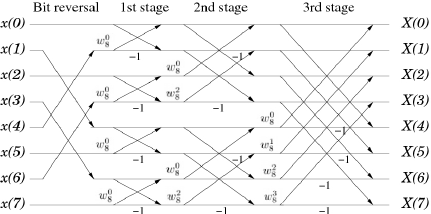
\includegraphics [scale=0.7]{bab2/img/bit-reverse-fft-butterfly}
	\caption {Bit-Reversal Butterfly FFT}
	\label {fig:bit-reverse-fft-butterfly}
\end{figure}

\begin{figure}
	\Centering
	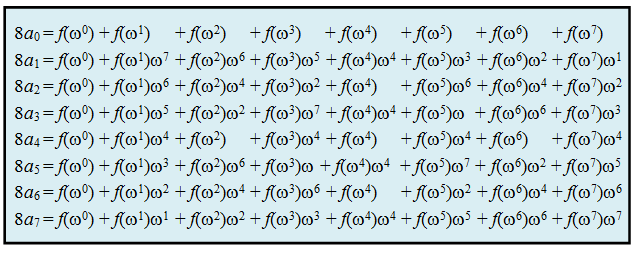
\includegraphics [scale=0.6]{bab2/img/inverse-fft}
	\caption {Inverse Transformasi Fourier Cepat}
	\label {fig:inverse-fft}
\end{figure}
Perhatikan bahwa \textit{Inverse Fast Fourier Transform} hampir sama dengan proses FFT, perbedaannya pada urutan serta $ \omega_N $.

\subsection{Number Theoretic Transform} \label{ssec:ntt}
\textit{Number Theoretic Transform} atau NTT didapatkan dengan megeneralisasikan DFT pada $ \mathbb{Z}/p\mathbb{Z} $. NTT biasanya digunakan dalam mengalikan 2 polinomial dalam modulo prima tertentu. Kelebihan NTT adalah tidak ada \textit{precision error} yang sering terjadi pada FFT, karena kalkulasinya menggunakan bilangan integer. Kelemahan utama dari NTT adalah kita hanya dapat mengimplementasikan NTT dengan modulo prima yang memenuhi $ p = k \cdot n + 1 $, dimana $ k $ dan $ n $ adalah konstanta tertentu. Sehingga mengimplementasikan NTT dengan bilangan prima acak memerlukan CRT \textit{(Chinese Remainder Theorem)}.

Pertama, $ \omega_N $ harus berada dalam $ \mathbb{Z}/p\mathbb{Z} $, sedemikian hingga memenuhi persamaan \eqref{eq:root_of_unity_in_z_pz}.
\begin{equation}
	\begin{aligned}
		\omega_N^N = 1 \Mod{P} \\
		P = k \cdot n + 1 \\
	\end{aligned}
	\label{eq:root_of_unity_in_z_pz}
\end{equation}
Menggunakan teorema \ref{theo:fermat_little_theorem}, maka terdapat \textit{primitive root} $ g $, dengan $ x $ dari $ 1 \text{ sampai } P-1 $ maka hasil dari $ g^x \Mod{P} $ berada didalam rentang $ [1,P-1] $ dengan urutan tertentu. Menurut persamaan \eqref{eq:root_of_unity_in_z_pz}, kita bisa mendapatkan $ P-1 = k \cdot n $\cite{ntt}. Sehingga 
$$ \omega_n = g^{k} \Mod{P} $$
dan kita bisa membuktikan bahwa
$$ \omega_n^n = g^{k \cdot n} = g^{P-1} \equiv 1 \mod{P} $$
$$ \omega_n^m \not\equiv 1 , m < n $$

Oleh karena itu $ \omega_n $ merupakan n\textit{-th primitive root of unity}, yang diperlukan DFT dengan panjang $ n $. Tahap dalam NTT sama seperti FFT pada umunya, perbedaanya hanya pada nilai $ \omega_n $. Nilai dari $ g $ atau generator dapat dilakukan dengan memfaktorkan nilai $ P - 1 $ untuk mendapatkan faktor prima yang unik yang disebut $ upf $. Setelah mendapatkan $ upf $, $ g $ adalah generator apabila memenuhi persamaan \eqref{eq:criteria_of_generator}.
\begin{equation}
	g = \{ a^{\frac{N-1}{p}} \not\equiv 1 \mod{P} | a \in (1,N) , \text{for each } p \text{ in } upf \}
	\label{eq:criteria_of_generator}
\end{equation} 

Perhitungan NTT memerlukan banyak sekali perkalian modular dengan modulo tetap, oleh karena itu NTT dapat diimplementasikan dengan perkalian modular \textit{Montgomery}, untuk mempercepat aritmatika modular dalam NTT.

\subsection{Chinese Remainder Theorem}
\textit{Chinese Remainder Theorem} atau CRT merupakan sebuah teorema dalam teori bilangan yang dikembangkan oleh Sunzi pada tahun 201 - 300.
\begin{theo}[Chinese Remainder Theorem]
	\label{theo:chinese_remainder_theorem}
	Diberikan pasangan bilangan yang saling \textit{coprime} $n_1, n_2, \cdots, n_k$ dan sembarang bilangan $ a_1, a_2, \cdots, a_k $, dengan sistem konguensi 
	\begin{equation}
		\begin{aligned}
		x &\equiv a_1 \Mod{n_1}\\
		x &\equiv a_2 \Mod{n_2}\\
		& \vdots\\
		x &\equiv a_k \Mod{n_k}\\
		\end{aligned}
	\end{equation}
	mempunyai solusi, dan solusi adalah unik dalam modulo $ N = n_1n_2\cdots n_k$.
\end{theo}
Bedasarkan teorema \ref{theo:chinese_remainder_theorem}, bisa disusun langkah dalam menyelesaikan sistem kongruensi\cite{brilliant_crt}. 
\begin{enumerate}
	\item Hitung $ N = n_1 \times n_2 \times \cdots \times n_k$.
	\item Untuk setiap $ i = 1,2,\cdots,k $ hitung $$ y_i = \frac{N}{n_i} $$.
	\item Untuk setiap $ i = 1,2,\cdots,k $ hitung $ z_i = y_i^{-1} \mod{n_i} $
	\item Solusi sistem kongruensi adalah integer $ x = \sum_{i=1}^{k} a_i y_i z_i $, dengan $ x \mod{N} $ adalah solusi unik dari modulo $ N $
\end{enumerate}
Terdapat \textit{case} khusus dalam menyelesaikan sistem kongruensi dengan $ k = 2 $.
$$ x \equiv a_1 \Mod{n_1} $$
$$ x \equiv a_2 \Mod{n_2} $$
dengan $ n_1 \text{ dan } n_2 $ saling \textit{coprime}.
Menggunakan \textit{Bézout's identity} yang mengatakan bahwa terdapat dua bilangan $ m_1 \text{ dan } m_2 $ sehingga 
\begin{equation}
	m_1 n_1 + m_2 n_2 = 1.
	\label{eq:bezeout_identity}
\end{equation}
Sehingga solusi sistem kongruensi diberikan $ x = a_1 m_2 n_2 + a_2 m_1 n_1 $, dapat diubah menjadi persamaan \eqref{eq:crt_2_modulo}.
\begin{equation}
	\begin{aligned}
		x &= a_1 m_2 n_2 +a_2 m_1n_1 \\
		  &= a_1 (1-m_1 n_1) + a_2 m_1 n_1 \\
		  &= a_1 +( a_2-a_1) m_1 n_1.
	\end{aligned}
	\label{eq:crt_2_modulo}
\end{equation}

\subsection{Polinomial}
Dalam matmatika, polinomial atau suku banyak merupakan jumlah dari beberapa perkalian dari sebuah variabel konstan dengan koefisiennya\cite{}. Secara umum polinomial dinyatakan seperti persamaan \label{eq:persamaan_umum_polinomial}
\begin{equation}
	f_n(x) = \sum_{i=0}^{n} a_i x^i = a_n x^n + a_{n-1}^{n-1} + \cdots + a_2x^2 + a_1x + a_0
	\label{eq:persamaan_umum_polinomial}
\end{equation}
Pangkat tertinggi dari variabel $ x $ dari fungsi polinomial disebut dengan order/derajat dari polinomial.

\subsubsection{Pertambahan dan Pengurangan Polinomial}
Polinomial juga bisa diterapkan operasi pertambahan dan pengurangan dalam aritmatika. 
Didefinisikan 2 buah polinomial $f(x)$ dan $g(x)$ sebagai berikut.
$$ f(x) = a_n x^n + a_{n-1}^{n-1} + \cdots + a_2x^2 + a_1x + a_0 $$
$$ g(x) = b_m x^m + b_{m-1}^{m-1} + \cdots + b_2x^2 + b_1x + b_0 $$
Pada umumya operasi pertambahan polinomial $ f(x) + g(x) $ dinyatakan seperti dalam persamaan \eqref{eq:persamaan_tambah_polinomial}.
\begin{equation}
	f(x) + g(x) = \sum_{i=0}^{max(n,m)} (a_i + b_i) x^i
	\label{eq:persamaan_tambah_polinomial} 
\end{equation}
Kemudian operasi pengurangan polinomial $ f(x) - g(x) $ dinyatakan seperti dalam persamaan \eqref{eq:persamaan_kurang_polinomial}.
\begin{equation}
	f(x) - g(x) = \sum_{i=0}^{max(n,m)} (a_i - b_i) x^i
	\label{eq:persamaan_kurang_polinomial} 
\end{equation}
Secara umum kompleksitas operasi pertambahan dan pengurangan dari polinomial adalah $ \mathcal{O}{(max(n,m))} $ dengan $ n , m $ adalah derajat polinomial $ f(x) \text{ dan } g(x) $.

\subsubsection{Perkalian Polinomial}
Selain pertambahan dan pengurangan, polinomial juga terdapat operasi perkalian.
Didefinisikan 2 buah polinomial $f(x)$ dan $g(x)$ sebagai berikut.
$$ f(x) = a_n x^n + a_{n-1}^{n-1} + \cdots + a_2x^2 + a_1x + a_0 $$
$$ g(x) = b_m x^m + b_{m-1}^{m-1} + \cdots + b_2x^2 + b_1x + b_0 $$
Pada umumnya operasi perkalian polinomial $ f(x) \cdot g(x) $ dinyatakan seperti dalam persamaan \eqref{eq:persamaan_kali_polinomial}.
\begin{equation}
	f(x) \cdot g(x) = \sum_{i=0}^{n} \sum_{j=0}^{m} (a_i * b_j) x^{i+j}
	\label{eq:persamaan_kali_polinomial}
\end{equation}
Secara umum kompleksitas operasi perkalian polinomial adalah $ \mathcal{O}{(nm)} $ dengan $ n , m $ adalah derajat polinomial $ f(x) \text{ dan } g(x) $.

Operasi perkalian polinomial dapat dioptimasi menggunakan \textit{Number Theoretic Transform} \ref{ssec:ntt}. Langkah langkah untuk mengalikan polinomial $f(x)$ dan $g(x)$ (konvolusi) dalam modulo $ P $ adalah sebagai berikut :
\begin{enumerate}
	\item \textbf{Preproses} Melakukan penambahan nilai 0 pada polinomial $ f(x) $ atau $ g(x) $ apabila polinomial tersebut tidak memiliki derajat dari hasil pangkat dua.
	\item \textbf{Evaluasi NTT} Melakukan evaluasi NTT dari polinomial $ f(x) $ dengan \textit{roots of unity}.
	\item \textbf{Evaluasi NTT} Melakukan evaluasi NTT dari polinomial $ g(x) $ dengan \textit{roots of unity}.
	\item \textbf{Perkalian Titik} Melakukan perkalian titik sehingga $ h(x) = f(x)g(x) $.
	\item \textbf{Interpolasi NTT / Inversi NTT} Melakukan interpolasi titik menggunakan inversi NTT dari $ h(x) $ untuk mendapatkan polinomial dalam representasi koefisien kembali.
\end{enumerate}

\subsubsection{Pembagian Polinomial}
Didefinisikan 2 buah polinomial $f(x)$ dan $g(x)$ sebagai berikut.
$$ f(x) = a_n x^n + a_{n-1}^{n-1} + \cdots + a_2x^2 + a_1x + a_0 $$
$$ g(x) = b_m x^m + b_{m-1}^{m-1} + \cdots + b_2x^2 + b_1x + b_0 $$
dimana kita ingin menghitung polinomial $ f(x) $ dibagi oleh $ g(x) $, pembagian ini akan menghasilkan dua polinomial baru $ q(x) $ sebagai hasil bagi dan $ r(x) $ sebagai sisa hasil bagi. Sisa hasil bagi polinomial memiliki beberapa sifat khusus seperti dalam teorema \ref{theo:teorema_sisa_poli}.
\begin{theo}[Teorema Sisa Polinomial]
	\label{theo:teorema_sisa_poli}
	Bentuk umum pembagian polinomial adalah $ F(x) = P(x) \cdot H(x) + S(x) $ \\
	$ F(x) $ = polinomial awal \\
	$ P(x) $ = polinomial pembagai \\
	$ H(x) $ = polinomial hasil bagi \\
	$ S(x) $ = polinomial sisa \\
	\begin{enumerate}
		\item Jika polinomial $ F(x) $ berderajat $ n $ dibagi oleh $ (x - k) $ maka sisanya adalah $ F(k) $.
		\item Jika polinomial $ F(x) $ berderajat $ n $ dibagi oleh $ (ax - b) $ maka sisanya adalah $ F(\frac{b}{a}) $.
		\item Jika polinomial $ F(x) $ berderajat $ n $ dibagi oleh $ (x - a)(x - b) $ maka sisanya adalah $ \frac{F(a) - F(b)}{a - b} +  \frac{aF(a) - bF(b)}{a - b}$.
	\end{enumerate}
\end{theo}
Pada umumnya pembagian polinomial dapat dilakukan dengan pembagian secara klasik maupun dengan metode \textit{Horner}, akan tetapi kedua cara tersebut memiliki kompleksitas yang tinggi, oleh karena itu diperlukan algoritma lain dengan kompleksitas lebih rendah. Iterasi Newton dan \textit{Middle Product Optimization} merupakan dua algoritma yang bisa digunakan dalam pembagian polinomial.

\paragraph{Iterasi Newton}\mbox{}\\
\indent Misalkan terdapat 2 buah polinomial $f(x)$ dan $g(x)$ dalam $ \mathbb{Z}/p\mathbb{Z} $ sebagai berikut.
$$ f(x) = a_{2n-2} x^{2n-2} + \cdots + a_2x^2 + a_1x + a_0 $$
$$ g(x) = b_{n-1} x^{n-1} + \cdots + b_2x^2 + b_1x + b_0 $$
dan kita ingin membagi $ f $ dengan $ g $ sehingga $ f = qg + r $.
Misalkan 
$$ f^*(x) = x^{2n-2}f(1/x) = a_0 x^{2n-2} + \cdots + a_{2n-2} $$
$$ g^*(x) = x^{n-1}g(1/x) = b_0 x^{n-1} + \cdots + b_{n-1} $$
sehingga $ f^* $ dan $ g^* $ merupakan polinomial dengan urutan terbalik dari $ f $ dan $ g $, kemudian
$$  f(x) = q(x)g(x) + r(x) \iff f^*(x) = q*(x) q*(x) + x^{n-1+\lambda} r*(x) $$
dengan $ \lambda \geq 1 $. Jika kita bisa mencari nilai $ q* $ maka kita kita menghitung nilai dari sisanya atau $ r* $ dengan $ f-qg $.

Iterasi newton merupakan algortima iteratif untuk mengaproksimasi solusi dari fungsi non-linear $ f(x) = 0 $. Iterasi dimulai dengan dugaan awal nilai tertentu, yang konvergen dengan fungsi $ f(x) $. 
Didefinisikan \textit{Power series} $ \bar{p}(x) $ adalah aproksikmasi polinomial derajat $ n $ dari $ p(x) $ jika $ \bar{p}(x) = P(x) + O(x^n) = p(x) \mod{x^n} $. 
Misal $ y(x) = g(x)^{-1} $. Mencari $ y(x) $ ekivalen dengan mencari solusi dari persamaan $$ a(x) - \frac{1}{y(x)} = 0. $$

Didefinisikan $ f(y) = a(x) - \frac{1}{y} $, serta $ f(y_k) + f^{'}(y_k)(Y_{k+1} - y_k) = 0 $, maka dihasilkan persamaan \eqref{eq:persamaan_iterasi_newton}.
\begin{equation}
	\begin{aligned}
		y_{k+1} &= y_k - \frac{f(y_k)}{f^{'}(y_k)} \\
				&= y_k - \frac{a(x) - \frac{1}{y_k}}{\frac{1}{y_k^2}} \\
				&= y_k + y_k(1 - y_k \cdot a(x)).
	\end{aligned}
	\label{eq:persamaan_iterasi_newton}
\end{equation}
Untuk mencari nilai dari $ q* $, diawali dengan mencari nilai dari $ \frac{1}{g(x)} $, menggunakan iterasi newton memerlukan nilai awal $ y_0 = \frac{1}{g_{n-1}} $ atau inverse dari konstant, kemudian dilanjutkan untuk $ k $ dari $ 1 $ hingga $ \log_2 n $ menggunakan persamaan \eqref{eq:iterasi_newton}.
\begin{equation}
	y_k \equiv 2y_{k-1} - y_{k-1}^2 b^* \mod{x^{2^{k}}}
	\label{eq:iterasi_newton}
\end{equation}
Sehingga untuk menghitung nilai dari $ q* $ dapat menggunakan persamaan \eqref{eq:q_star}.
\begin{equation}
	q^* = f^* \cdot \frac{1}{g^*} \mod{x^n}
	\label{eq:q_star}
\end{equation}
Sehingga pada setiap step memerlukan 3 kali perkalian polinomial dan 1 kali perkalian polinomial untuk mendapatkan nilai dari $ q* $. Untuk mendapatkan nilai dari $ r $ menggunakan persamaan $ r = f-gq $ memerlukan 1 kali perkalian polinomial kembali. Sehingga iterasi newton memerlukan banyak sekali perkalian polinomial. Selanjutnya akan dibahas mengenai optimasi untuk menurunkan ukuran dari perkalian polinomial.

\paragraph{Middle Product Optimization} \mbox{}\\
\indent Misal $ n = 2^k $, kemudian diketahui bahwa
$$ y_k \equiv 2y_{k-1} - y_{k-1}^2 b^* \mod{x^{2^{k}}} = y_{k-1} + y_{k-1}(1 - b^* y_{k-1}) \mod{x^{2^k}}. $$
Dalam keadaan normal, perkalian polinomial dengan derajat $ 2n - 1 $ dan $ n - 1 $ memerlukan perkalian polinomial berbasis NTT memerlukan \textit{array} yang bisa menampung setidaknya $ 3n $ elemen. Tetapi perkalian polinomial berbasis NTT memerlukan input dengan ukuran pangkat dua, sehingga memerlukan \textit{array} dengan ukuran $ 4n $. Mengetahui bahwa $ 1-y_kb^* \equiv 0 \mod{x^{2^k}} $, sehingga perkalian $ y_kb^* $ akan menghasilkan polinomial seperti dalam persamaan \eqref{eq:persamaan_asal_mula_m(x)}, dengan $ h(x) = 1 + 0 \cdot x + \cdots + 0 \cdot x^{n-1}. $
\begin{equation}
	\begin{aligned}
y_k \cdot b^* &= h(x) + m_0 \cdot x^n + m_1 \cdot x^{n+1} + \cdots + m_n-1 \cdot x^{2n-1} + O(x^{2n}) \\
			  &= h(x) + x^n ( m_0 + m_1 \cdot x + \cdots + m_n-1 \cdot x^{n-1}) + O(x^{2n}) \\
			  &= h(x) + x^n m(x) + (c_0 + c_1 \cdot x + \cdots + c_{n-1} \cdot x^{n-1} ) \\
	\end{aligned}
	\label{eq:persamaan_asal_mula_m(x)}
\end{equation}
$$ \text{dimana } m(x) = m_0 + m_1 \cdot x + \cdots + m_n-1 \cdot x^{n-1}. $$

Sehingga bisa didefinisikan \textit{field} $ F $ dan polinomial $ a(x) $ yang merupakan \textit{power series} dalam $ F[[x]] $ dengan $ a_0 \neq 0 $. Untuk sembarang integer $ n \geq 2 $, misal $ b = a(x) \mod{x^n} $, dan $ y = a(x)^{-1} \mod{x^m} $ dengan $ m = \lceil \frac{n}{2} \rceil $. Jika 
$$ y \cdot b = \sum_{i=0}^{n+m-2}g_ix^i, $$ maka polinomial $$ \sum_{i=0}^{n-m+1} g_{m+i} x^i $$ disebut dengan \textit{Middle Product}.
Menggunakan definisi diatas, dapat didefinisikan teorema \ref{theo:middle_product}\cite{middle_product_op}.

\begin{theo}[Middle Product]
	\label{theo:middle_product}
	Misal $ F,a(x),n,b,m \text{ dan } y $ sama seperti definisi diatas, serta $ N $ adalah bilangan pangkat 2 sehingga $ N/2 < n \leq N $ dan $ \omega $ merupakan \textit{N-th primitive root of unity}. Jika
		$$ FFT(b,N,\omega) = (B_0, B_1, \cdots, B_{N-1}), $$
		$$ FFT(y,N,\omega) = (Y_0, Y_1, \cdots, Y_{N-1}), $$
		$$ D_i = B_i \cdot Y_i \text{ untuk i } = 0, \cdots N-1 \text{ dan } $$
		$$ (d_0, d_1, \cdots , d_{N-1}) = N^{-1} FFT(\sum_{i=0}^{N-1} D_iX^i, N, \omega^-1), \text{ sehingga } $$
		$$ \text{MP } = \sum_{i=0}^{n-m+1} d_{m+i}x^i. $$
		\label{eq:middle_product}
\end{theo}

Optimasi ini mengurangi jumlah pemanggilan FFT/NTT dengan mengurangi ukuran \textit{array} pada perkalian FFT/NTT dari $ 2n $ menjadi $ n $.

\section{Strategi Penyelesaian Permasalahan FACTMODP dengan Multipoint Evaluation}
Pada subbab ini akan dipaparkan mengenai strategi penyelesaian masalah klasik pada daring SPOJ dengan kode FACTMODP. Secara singkat, strategi penyelesaian masalah dari FACTMODP menggunakan Multipoint Evaluation terbagi menjadi 4 bagian besar yaitu :
\begin{enumerate}
	\item Perumusan Transformasi Faktorial
	\item Membangun Pohon Polinomial
	\item Evaluasi Pohon Polinomial
	\item Komputasi Faktorial bedasarkan Hasil Evaluasi
\end{enumerate}

Sebagai contoh, pada subbab ini akan menggunakan parameter $ N = 10 $ serta $ P = 10^9 + 7 $. Nilai $ N $ dan $ P $ yang dipilih berada didalam batasan yang didefinisikan dalam subbab \ref{sec:batasan_masalah}. Persoalan utama dalam tugas akhir ini adalah memodelkan faktorial sedemikian hingga dapat dikomputasi dengan kompleksitas dibawah $ \mathcal{O}{(N)} $.

\subsection{Perumusan Transformasi Faktorial}
\label{sec:perumusan_transformasi_faktorial}
Misal $ v = \lfloor \sqrt{N} \rfloor $ dan polinomial $ g(x) = \prod_{i=0}^v (x + vi + 1) $, sehingga bisa didefinisikan persamaan \eqref{eq:persamaan_faktorial_baru}
\begin{equation}
	N ! = \left( \prod_{i=0}^{v-1} g(i) \right) \cdot \prod_{i=v^2+1}^n i
	\label{eq:persamaan_faktorial_baru}
\end{equation}
Untuk $ N = 10 $, maka $$ g(x) = (x+1)(x+4)(x+7) = (x^3 + 12x^2 + 39x + 28). $$
Menggunakan \textit{Multipoint Evaluation}, nilai $ g(0), g(1), \cdots , g(v) $ dapat dievaluasi sekaligus, sehingga komputasi $ N! \text{ mod } P $ memiliki kompleksitas $ \mathcal{O}{(\sqrt{N}\ log^2 N )}. $
\begin{theo}[Wilson's Theorem]
	\label{theo:wilson}
	Jika terdapat bilangan asli $ p > 1 $ adalah bilangan prima, maka hasil perkalian dari semua bilangan bulat positif yang kurang dari n ditambah 1 adalah kelipatan dari $ p $. Sehingga dalam notasi kongruen dapat didefinisikan persamaan \eqref{eq:wilson_theorem}.
	\begin{equation}
		(p - 1)! \equiv -1 \Mod{p}
		\label{eq:wilson_theorem}
	\end{equation}
\end{theo}



Dengan menggunakan teorema \ref{theo:wilson}, komputasi $ N! $  mod $ P $ memiliki kompleksitas $ \mathcal{O}{(\sqrt{min(N,P-N-1)}\ log^2 (min(N,P-N-1)) )}$.

\subsection{Membangun Pohon Polinomial}
\label{sec:membangun_pohon_polinomial}
Membangun pohon polinomial merupakan tahap selanjutnya setelah kita menemukan polinomial $ g(x) $. Pada tahap ini kita akan membangun pohon polinomial yang menjadi dasar dalam \textit{Multipoint Evaluation}. Misal $ u_0, u_1, \cdots , u_{n-1} $ adalah titik yang akan dievaluasi pada polinomial $ g(x) $. Untuk membangun pohon polinomial, kita dapat menggunakan polinomial $( x - u_i) $ untuk $ 0 \leq i < n $ sebagai \textit{leaves}.

Setiap \textit{node} dalam pohon dilambangkan dengan $ M_{i,j} $ yang menyatakan \textit{node} dengan tinggi $ i $ dan \textit{node} ke-$j$ dari kiri pohon, dan perkalian semua \textit{node} atau \textit{leaves} dibawah \textit{node} tersebut seperti pada gambar \ref{fig:ilustrasi-pohon-polinomial}. 

\begin{figure}
	\Centering
	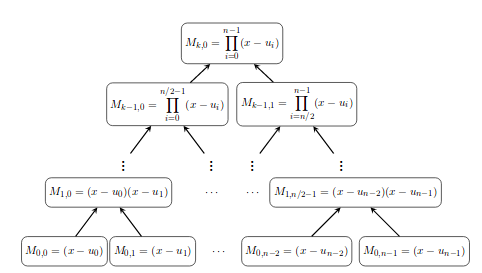
\includegraphics [scale=0.5]{bab2/img/ilustrasi-pohon-polinomial}
	\caption {Ilustrasi Pohon Polinomial}
	\label {fig:ilustrasi-pohon-polinomial}
\end{figure}

Pseudocode \ref{psdo:general_subproduct_tree} menjelaskan secara umum dalam membangun pohon polinomial yang digunakan sebagai dasar dari \textit{Multipoint Evaluation}.

\begin{algorithm}
	\caption{Membangun Pohon Polinomial (General)}
	\label{psdo:general_subproduct_tree}
	\begin{algorithmic}[1]
		\Require $ N = 2^k, k \in \mathbb{N},\ u_0, u_1, \cdots , u_{n-1} \in R $
		\Ensure $ \text{Pohon Polinomial } M_{i,j} \text{ untuk } 0 \leq i \leq k \text{ dan } 0 \leq j < 2^{k-i} $
		\For {$ j = 0, \cdots , n-1 $} $ M_{0,j} \gets (x - u_i) $ \EndFor
		\For {$ i = 1, \cdots , k $ }
			\For {$ j = 0, \cdots, 2^{k-i}-1 $} $ M_{i,j} \gets M_{i-1,2j} \cdot M_{i-1,2j+1}$ \EndFor
		\EndFor
	\end{algorithmic}
\end{algorithm}
Sehingga \textit{root} dalam tree menampung nilai $ M_{k,0} = \prod_{i=0}^{n-1} (x - u_i) $. Pseudocode \ref{psdo:general_subproduct_tree} diatas merupakan pseudocode secara general yang berlaku apabila $ N $ merupakan bilangan pangkat dua, apabila $ N $ bukan bilangan pangkat dua, kita bisa menerapkan algoritma rekursi dengan mengalikan sisanya dengan polinomial $ 1 $, yang dibahas pada bab berikutnya. Sehingga untuk $ N = 10 $, maka pohon polinomial akan terlihat seperti dalam gambar \ref{fig:pohon-polinomial-n-10}.
\begin{figure}
	\Centering
	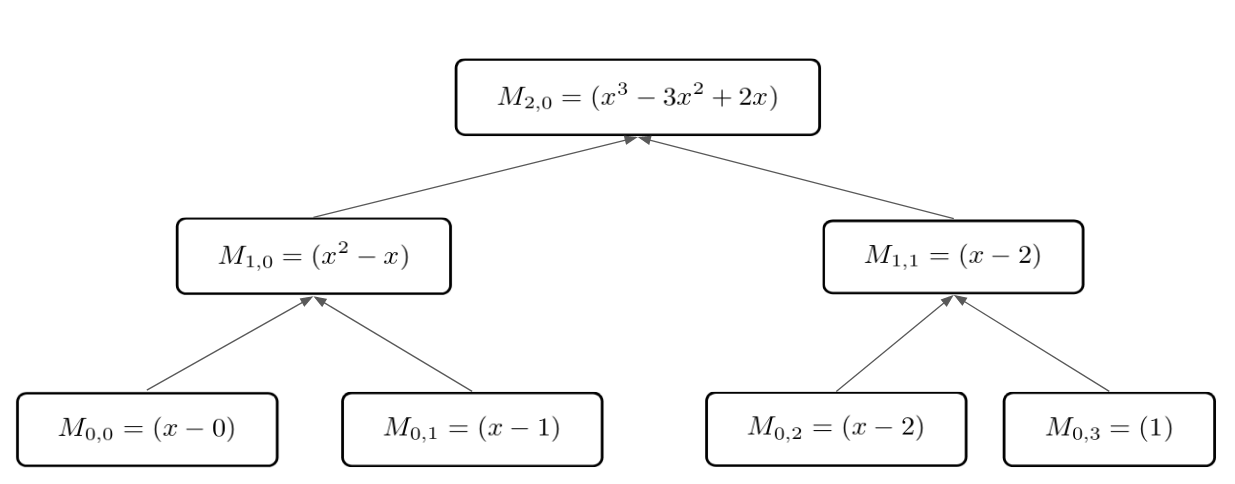
\includegraphics [scale=0.25]{bab2/img/pohon-polinomial-n-10}
	\caption {Pohon Polinomial untuk $ N  = 10 $}
	\label {fig:pohon-polinomial-n-10}
\end{figure}

\subsection{Evaluasi Pohon Polinomial}
\label{sec:evaluasi_pohon_polinomial}
Setelah pohon polinomial terbentuk, kita dapat menjalankan algoritma \textit{Multipoint Evaluation}. Algoritma ini merupakan algoritma dengan tipe \textit{divide-and-conquer} menggunakan \textit{Chineese Remainder Theorem}. Misal $ R  = \mathbb{Z}_p $, $ f = g(x) $ dan untuk $ 0 \leq i < n $, $ m_i = z - u_i $, maka terdefinisikan homomorfisme ring surjektif 
\begin{equation}
	\begin{aligned}
		\phi_i : R \longrightarrow R/<m_i>, \\
		\phi_i(f) : f \text{ mod } m_i.
	\end{aligned}
\end{equation}
sehingga berlaku homomorfisme ring surjektif baru,
\begin{equation}
	\begin{aligned}
		\phi_i : R \longrightarrow R/<m_0> \times \cdots \times <m_{n-1}>, \\
		\phi_i(f) : f \text{ mod } m_0, \cdots f \text{ mod } m_{n-1} 
	\end{aligned}
	\label{eq:ring_of_homomorfisme_2}
\end{equation}

Menggunakan teorema \ref{theo:teorema_sisa_poli}, ketika membagi $ f $ dengan $ (x - u_i ) $, sama dengan hasil dari $ f(u_i) $ yaitu 
\begin{equation}
	\begin{aligned}
		f(u_i) &= q(u_i) \cdot m_i(u_i) + r(u_i) \\
			   &= q(u_i).0 + r(u_i) \\
			   &= r(u_i) \\
			   &= f \text{ mod } (x - u_i)
	\end{aligned}
	\label{eq:f_mod_ui}
\end{equation}

Persamaan \eqref{eq:f_mod_ui} dan \eqref{eq:ring_of_homomorfisme_2} merupakan dasar dari metode evaluasi polinomial dengan $ n $ titik. Tetapi pembagian polinomial berderajat $ n-1 $ dengan $ n $ mono polinomial memiliki kompleksitas $ \mathcal{O}{(n^2)} $, sehingga kita bisa menggunakan polinomial dengan ukuran lebih besar. Disinilah pohon polinomial berperan, daripada membagi $ f $ dengan \textit{leaves} dari pohon, lebih baik membagi $ f $ tiap level dari pohon. Pertama misalkan
\begin{equation}
	\begin{aligned}
		r = f \text{ mod } \prod_{i=0}^{n-1} (x-u_i) = M_{k,0} \\
	\end{aligned}
\end{equation}

Untuk setiap level berikutnya, $ r $ akan menjadi $ f $ baru pada setiap \textit{node} nya dan menghitung $ r $ kembali. Karena pohon polinomial merupakan pohon biner, maka jumlah pembagian polinomial untuk menghitung evaluasi berkurang dari $ \mathcal{O}{(n^2)} $ menjadi $ \mathcal{O}{(log \ n)} $. \textit{Multipoint Evaluation} merupakan algoritma gabungan dari Membangun Pohon Polinomial pada subbab \ref{sec:membangun_pohon_polinomial} dan Evaluasi Pohon Polinomial pada subbab \ref{sec:evaluasi_pohon_polinomial}.
\begin{algorithm}
	\caption{Evaluasi Pohon Polinomial (General)}
	\label{psdo:general_evaluasi_pohon_polinomial}
	\begin{algorithmic}[1]
		\Require $ N = 2^k, k \in \mathbb{N},f \in R[x] \text{ dan pohon polinomial } M_{i,j}  $
		\Ensure $ f(u_0), \cdots , f(u_{n-1}) $
		\State $ r \gets f \text{ mod } M_{k,0} $
		\State panggil fungsi dengan input $ r, n/2 $ dan pohon dengan root $ M_{k-1,0} $
		\State panggil fungsi dengan input $ r, n/2 $ dan pohon dengan root $ M_{k-1,1} $ \\
		\Return $ r(u_0), \cdots , r(u_{n-1})) $
	\end{algorithmic}
\end{algorithm}

Menggunakan pseudocode \ref{psdo:general_evaluasi_pohon_polinomial}, untuk $ N = 10 $ maka didapatkan hasil seperti gambar \ref{fig:evaluasi-pohon-n-10}.

\begin{figure}
	\Centering
	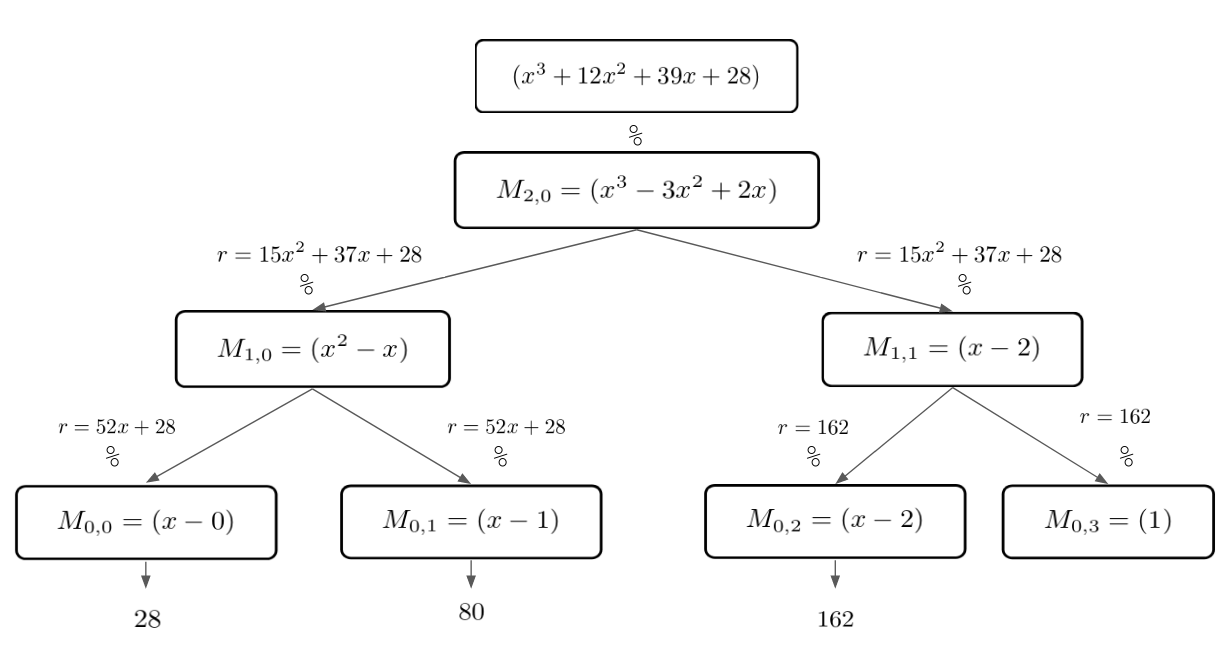
\includegraphics [scale=0.25]{bab2/img/evaluasi-pohon-n-10}
	\caption{Evaluasi pada Pohon Polinomial untuk $ N = 10 $}
	\label{fig:evaluasi-pohon-n-10}
\end{figure}


\subsection{Komputasi Faktorial bedasarkan Hasil Evaluasi}
Mengacu pada subbab \ref{sec:perumusan_transformasi_faktorial}, didapatkan rumus faktorial sebagai berikut.
$$ N ! = \left( \prod_{i=0}^{v-1} g(i) \right) \cdot \prod_{i=v^2+1}^n i $$

Setelah mendapatkan nilai dari $ g(0), g(1), \cdots, g(v-1) $, kita bisa mendapatkan nilai dari $ N! $, dengan mengalikan nya dengan $ \prod_{i=v^2+1}^n i $. Pada subbab \ref{sec:perumusan_transformasi_faktorial}, telah disinggung tentang teorema \ref{theo:wilson} yang dapat menurunkan kompleksitas perhitungan. Penggunaan teorema \ref{theo:wilson}, dalam contoh $ N = 9 $ dan $ P = 13 $, nilai $ 12! \equiv -1 \mod{13} $, sehingga dalam menghitung $ 10! $ menggunakan teorema \ref{theo:wilson}, 
$$ 9! \equiv \frac{-1}{12 \cdot 11 \cdot 10} \mod{13} $$
$$ 9! \equiv \frac{-1}{-1 \cdot -2 \cdot -3} \mod{13} $$

Sehingga persamaan \eqref{eq:persamaan_faktorial_baru}, bisa diubah menjadi persamaan \eqref{eq:rumus_faktorial_baru2}
\begin{equation}
	N! \equiv
	\begin{cases}
		\left( \displaystyle\prod\limits_{i=0}^{v-1} g(i) \right) \cdot \displaystyle\prod\limits_{i=v^2+1}^n i \mod{P}, 	      & \text{if } 2N < P \\\\
		\dfrac{1}{\left( \displaystyle\prod\limits_{i=0}^{v-1} g(i) \right) \cdot \displaystyle\prod\limits_{i=v^2+1}^n i} \mod{P}
		& \text{if } 2N >= P \text{ dan } M \text{ genap}\\\\
		P -\dfrac{1}{\left( \displaystyle\prod\limits_{i=0}^{v-1} g(i) \right) \cdot \displaystyle\prod\limits_{i=v^2+1}^n i} \mod{P}
		& \text{if } 2N >= P \text{ dan } M \text{ ganjil} \\
	\end{cases}
	\label{eq:rumus_faktorial_baru2}
\end{equation}
$$ \text{ dengan } M = P-N-1 $$

\section {Strategi Penyelesaian Umum}
Tujuan permasalahan ini adalah membuat sepasang nilai \textit{signature (r, s)} menurut prosedur yang dijelaskan. Berdasarkan prosedur pada subbab \ref{sec:Keluaran Permasalahan}, beberapa variabel disebutkan, diantaranya $q$, $p$, $g$, $Hm$, $k$, $r$, $s$, dan $x$. Untuk variabel $q$, $p$, $g$, dan $Hm$, nilai variabel tersebut telah diberikan oleh soal sebagai parameter masukan. Untuk variabel $k$, $r$, dan $s$, nilai variabel tersebut terbentuk seiring proses \textit{signing}. Hanya nilai $x$ yang tidak diberikan oleh soal maupun tidak terdefinisi pada prosedur \textit{signing}. Namun untuk nilai $x$, soal memberikan penjelasan bagaimana nilai $x$ terbentuk.
\begin{enumerate}
\item Tentukan nilai $x$ secara acak dimana $0 < x < q$.
\item Hitung $y = g^x\ mod\ p$.
\item Nilai \textit{public key} adalah $(p, q, g, y)$. Nilai \textit{private key} adalah $x$.
\end{enumerate}
Untuk mampu membuat \textit{signature}, terlebih dahulu dicari nilai $x$ pada persamaan $y=g^x\ mod\ p$. Cara menemukan nilai $x$ pada persamaan tersebut akan dijelaskan pada subbab \ref{sec:Strategi Penyelesaian Logaritma Diskret}. Setelah menemukan nilai $x$, langkah selanjutnya cukup mengikuti proses yang dijelaskan pada soal.

Ringkasnya, permasalahan ini dapat diselesaikan dengan prosedur di gambar \ref{fig:main_diagram}.
\begin{figure}
	\Centering
	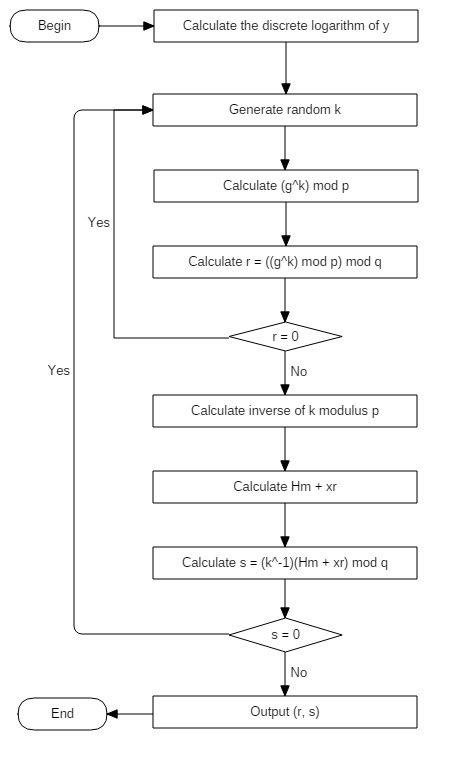
\includegraphics [scale=0.5]{bab2/img/main-diagram}
	\caption {Diagram Alur Penyelesaian Permasalahan}
	\label {fig:main_diagram}
\end{figure}
Terdapat beberapa \textit{bottleneck} pada prosedur pembuatan signature, di antaranya penghitungan logaritma diskret $ y $, penghitungan nilai $g^k\ mod\ p$, dan penghitungan invers $k\ \left(mod\ p\right)$. Selain proses yang telah dipaparkan pada gambar \ref{fig:main_diagram}, terdapat sebuah proses yang merentang di tiap tahapan pembuatan \textit{signature}.

Soal menyiratkan bahwa parameter $p$ memiliki nilai paling tinggi sekitar $2^{60}$ sedangkan pada waktu penulisan, nilai \textit{integer} yang paling besar yang dapat ditampung pada mesin adalah $2^{64}$. Konsekuensi tingginya parameter $p$ adalah akan ada parameter lain yang memiliki batas atas nilai yang tinggi pula. Hal ini dapat menyebabkan masalah pada saat melakukan perkalian.

Perkalian dua nilai yang mendekati $2^{60}$ dapat mengakibatkan \textit{integer overflow}. Maka pada proses perkalian di seluruh tahapan pembuatan \textit{signature}, prosedur perkalian harus menggunakan metode yang dapat menghindari \textit{integer overflow}.

Berdasarkan penjelasan yang telah dijabarkan, hal-hal yang diperlukan untuk menyelesaikan permasalahan DSA Attack adalah sebagai berikut.

\begin{enumerate}
	\item Strategi penghitungan logaritma diskret, akan dibahas pada subbab \ref{sec:Strategi Penyelesaian Logaritma Diskret}.
	\item Strategi pemangkatan modular (penghitungan nilai $ g^k\ mod\ p $), akan dibahas pada subbab \ref{sec:Strategi Penyelesaian Pemangkatan Modular}.
	\item Strategi penghitungan invers $ k\ \Mod{P} $, akan dibahas pada subbab \ref {sec:Strategi Penyelesaian Invers Modulus}.
	\item Strategi perkalian modular (penghitungan nilai $ a * b\ mod\ p $), akan dibahas pada subbab \ref{sec:Strategi Perkalian Modular}.
\end{enumerate}

\section{Strategi Penyelesaian Pemangkatan Modular}
Bagian ini akan menjelaskan beberapa variasi penyelesaian pencarian hasil pemangkatan pada persamaan kongruen yang dijabarkan pada persamaan \eqref{eq:pemangkatan_modular}.
\begin{equation}
h \equiv a^k\ mod\ m,\text{untuk a, k, dan m yang ditentukan}
\label{eq:pemangkatan_modular}
\end{equation}

\subsection{Strategi Penyelesaian Pemangkatan Modular secara Naif}
Pencarian hasil persamaan \eqref{eq:pemangkatan_modular} dapat dicari secara iteratif. Hasil perkalian disimpan pada sebuah variabel sementara, $temp_h$. Nilai $temp_h$ secara berkala dikalikan dengan $a$ sebanyak $k$ kali. Setelah pemangkatan selesai dilakukan, nilai $temp_h$ dimodulus dengan $ m $. Prosedur ini ditunjukkan pada pseudocode \ref{psdo:modex_naive}.

\begin{figure}
\begin{lstlisting}[firstnumber=0]
NAIVE-MODULAR-EXPONENTIATION (a, k, m)
let temp_h = 1
for i = 1 to k
	temp_h = temp_h * a
	temp_h = temp_h mod m
return temp_h
\end{lstlisting}
\caption{Pseudocode Penyelesaian Pemangkatan Modular Secara Naif}
\label{psdo:modex_naive}
\end{figure}

Strategi ini membutuhkan $O(k)$ iterasi. Untuk nilai $k$ yang besar, metode ini tidak cukup baik untuk digunakan mengingat ada tahapan lain yang membutuhkan waktu komputasi yang tinggi. Untuk itu sebuah strategi alternatif akan diajukan pada subbab \ref{sec:Strategi Penyelesaian Pemangkatan Modular dengan Repeated Squaring}.

\subsection{Strategi Penyelesaian Pemangkatan Modular dengan Repeated Squaring}

Metode ini memanfaatkan representasi biner indeks pangkat $k$ dalam melakukan pemangkatan. Diberikan tiga masukan: \textit{generator}, \textit{exponent}, dan $p$ yang mengikuti persamaan \eqref{eq:pemangkatan_modular}.
\begin{equation}
	h \equiv generator^{exponent}\ mod\ p
	\label{eq:pemangkatan_modular_repeated_squaring}
\end{equation}
Gambar \ref{fig:repeated_squaring} menjabarkan prosedur metode ini.
\begin{figure}
	\Centering
	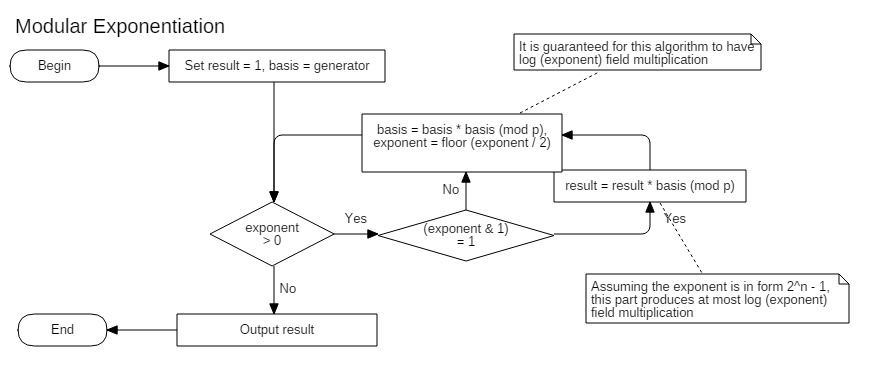
\includegraphics[scale=0.5,angle=90]{bab2/img/modular-exponentiation}
	\caption{Diagram Alur Pemangkatan Modular dengan \textit{Repeated Squaring}}
	\label{fig:repeated_squaring}
\end{figure}

Strategi ini memiliki kompleksitas $O\left(log_2\ p\right)$.

\subsection{Penjelasan Strategi Penyelesaian Pemangkatan Modular dengan Repeated Squaring}

Strategi ini berangkat dari perkalian berulang sebuah nilai $a$ (pada Gambar \ref{fig:repeated_squaring} dinotasikan dengan $ generator $) sebanyak $ k $ (pada Gambar \ref{rig:repeated_squaring} dinotasikan dengan $ exponent $) kali. Dengan kata lain, dibutuhkan $k$ proses perkalian dengan nilai $ a $. Hal ini ditunjukkan pada strategi pemangkatan modular naif. Kendati begitu, ada cara lain dimana walaupun proses pemangkatan membutuhkan $ k $ proses perkalian, pada praktiknya proses perkalian yang terjadi tidak sampai $ k $ kali.

Ide strategi ini adalah dengan memecah pemangkatan menjadi komponen yang lebih kecil. Pemecahan tersebut ditunjukkan pada persamaan \eqref{eq:dekomposisi_eksponen}.
\begin{equation}
a^q = a^{e_1} * a^{e_2} *\ldots*a^{e_n},\ \text{dimana}\ q=e_1+e_2+\ldots+e_n
\label{eq:dekomposisi_eksponen}
\end{equation}

Setelah ini akan dijelaskan mengenai nilai $e_i$. 

Pemangkatan memiliki sifat-sifat operasi layaknya aritmatika pada umumnya, dengan syarat basis pemangkatan harus sama. Strategi ini memanfaatkan sifat perkalian indeks pemangkatan seperti yang ditunjukkan pada persamaan \eqref{eq:dekomposisi_perkalian_indeks_pangkat}.
\begin{equation}
a^r = a^{s*t} = (a^s)^t
\label{eq:dekomposisi_perkalian_indeks_pangkat}
\end{equation}

Substitusi nilai $ s $ menjadi $ \frac{r}{2} $ dan $ t $ menjadi $2$.
\begin{equation}
a^r = a^{\frac{r}{2}*2} = (a^{\frac{r}{2}} )^2
\label{eq:substitusi_indeks_pangkat}
\end{equation}

Penghitungan nilai $ g^{\frac{r}{2}} $ dilakukan dengan menggunakan bentuk persamaan \eqref{eq:substitusi_indeks_pangkat}, hingga didapat nilai $ \displaystyle \frac{r}{2} = 1$. Perkalian secara rekursif ini memiliki jumlah perkalian mengikuti relasi rekurens berikut.
\begin{subequations}
	\[
		O(r)=
		\begin{cases}
			O(1), 			  & \text{if } r = 1 \\
			O(\frac{r}{2}+1), & \text{if } r > 1
		\end{cases}
		\tag{\ref{eq:rekurens_jumlah_perkalian}}
	\]
	\label{eq:rekurens_jumlah_perkalian}
\end{subequations}

Berdasarkan relasi rekurens \eqref{eq:rekurens_jumlah_perkalian}, jumlah perkalian yang dibutuhkan untuk melakukan pemangkatan dengan metode ini adalah $O(log_2\ r)$ dimana $r$ merupakan bilangan pangkat 2.

Telah dijelaskan bagaimana mencari hasil pangkat dimana indeks pangkat $r$ berupa bilangan pangkat 2. Metode pemangkatan dengan \textit{repeated squaring} juga dapat digunakan untuk mencari hasil pangkat dengan indeks pangkat $ r $ bukan bilangan pangkat 2. Pertama, representasi biner dari $ q $ dicari terlebih dahulu. Diberikan sebuah representasi biner r, $ \left\langle a_0,a_1,\cdots,a_n\right\rangle $ yang mengikuti persamaan \eqref{eq:dekomposisi_biner}.
\begin{equation}
r = (2^0 * r_0) + (2^1* r_1) + (2^2 * r_2) + \cdots + (2^n* r_n)
\label{eq:dekomposisi_biner}
\end{equation}

Nilai $ r $ pada persamaan \eqref{eq:dekomposisi_biner} kemudian dimasukkan ke $ a^r $ menjadi
\begin{align}
a^r &= a^{(2^0 * r_0) + (2^1 * r_1) + (2^2 * r_2) + \cdots + (2^n * r_n)} \\
a^r &= a^{2^0 * r_0} * a^{2^1 * r_1} * a^{2^2 * r_2} * \cdots * a^{2^n * r_n} \\ 
a^r &= (a^{2^0})^{r_0} * (a^{2^1})^{r_1} * (a^{2^2})^{r_2} * \cdots * (a^{2^n})^{r_n} \\
a^r &= (a^1)^{r_0} * (a^2)^{r_1} * (a^4)^{r_2} * \cdots * (a^{2^{log_2\ r}})^{r_n} \\
a^r &= y_0^{r_0} * y_1^{r_1} * y_2^{r_2} * \cdots * y_n^{r_n},\text{untuk } y_i=a^{2^i}
\label{eq:generalisasi_dekomposisi_biner_pemangkatan}
\end{align}

Persamaan \eqref{eq:generalisasi_dekomposisi_biner_pemangkatan} menunjukkan transformasi penghitungan pemangkatan dengan $ r $ menjadi sederet perkalian. Perlu diperhatikan bahwa penghitungan nilai $ (a^2)^i $ membutuhkan $ O(log_2\ 2^i) $ perkalian. Maka penghitungan $ y_i=a^{2^i} $ juga membutuhkan $ O(log_2\ 2^i) $ perkalian. Dari penjabaran ini, untuk menghitung semua nilai $ y_i $ pada persamaan \eqref{eq:generalisasi_dekomposisi_biner_pemangkatan} membutuhkan perkalian sebanyak
\begin{equation}
\sum_{i=1}^{n} log_2\ {2^i}=\sum_{i=1}^{n} i=\frac{n(n+1)}{2}
\label{eq:jumlah_perkalian_generalisasi_dekomposisi_biner}
\end{equation}

Perhatikan bahwa $ y_0 $ tidak diikutsertakan pada penghitungan karena $ y_0=a^{2^0}=a^1 $, sehingga tidak dibutuhkan perkalian apapun. Total perkalian yang dibutuhkan untuk menghitung $ y_i=a^{2^i} $ pada persamaan \eqref{eq:generalisasi_dekomposisi_biner_pemangkatan} adalah $ \frac{n(n+1)}{2} \in O(n^2) $. Metode ini tentu tidak lebih baik dari metode pemangkatan naif dimana dibutuhkan $ O\left(n\right) $ perkalian. Maka dari itu perlu dilakukan perubahan mengenai cara penghitungan $ y_i $.

Untuk menekan jumlah perkalian, penghitungan $ y_i $ dapat diubah menjadi relasi rekurens \eqref{eq:relasi_rekurens_y_i}.
\begin{subequations}
	\[
		y_i=
		\begin{cases}
			a, 		   & \text{if } i = 0 \\
			y_{i-1}*a, & \text{if } i > 0
		\end{cases}
		\tag{\ref{eq:relasi_rekurens_y_i}}
	\]
	\label{eq:relasi_rekurens_y_i}
\end{subequations}

Untuk mencari nilai $ y_i $, cukup menggunakan nilai $ y_{i-1} $ dan dikalikan dengan $ a $. Konsekuensi yang dimiliki cara ini adalah nilai $ y_i $ dapat digunakan untuk mendapatkan nilai $ y_{i+1} $. Maka sebetulnya untuk menghitung nilai $ y_i $, tidak perlu menghitung dari $ y_0 $. Apabila nilai $ y_{i-1} $ sudah diketahui, cukup mengalikan nilai tersebut dengan $ a $.

Pemanfaatan relasi rekurens \eqref{eq:relasi_rekurens_y_i} dapat dilakukan dengan menggunakan nilai $ y_i $ dan variabel $ temp $ yang berfungsi untuk menyimpan hasil perkalian. Mulai dari $ i=0 $, pangkatkan $ y_i $ dengan $ r_i $. Pemangkatan ini hanya memiliki dua hasil seperti yang ditunjukkan pada persamaan \eqref{eq:hasil_relasi_rekurens_y_i}.
\begin{subequations}
	\[f_y(i)=
		\begin{cases}
			1,  & \text{if } r_i=0 \\
			y_i,& \text{if } r_i=1
		\end{cases}
		\tag{\ref{eq:hasil_relasi_rekurens_y_i}}
	\]
	\label{eq:hasil_relasi_rekurens_y_i}
\end{subequations}
Hasil pemangkatan (yaitu nilai $ f_y(i) $) digabungkan ke $ temp $ dengan cara dikalikan.

Dari penjabaran tersebut, penghitungan persamaan \eqref{eq:generalisasi_dekomposisi_biner_pemangkatan} dengan metode ini membutuhkan hanya satu kali perhitungan nilai $ y_i $, yaitu penghitungan $ y_i $ pada $ i=n $. Proses penghitungan $ y_n $ juga menghitung nilai $ y_0 $ hingga $ y_{n-1} $. Sehingga dengan menghitung $ y_n $, nilai $ y_0 $ hingga $ y_{n-1} $ juga didapat. Jumlah perkalian menggunakan relasi rekurens \eqref{eq:relasi_rekurens_y_i} adalah $ O(n) $ dimana $ n=log_2\ r$ untuk sebuah indeks pangkat $ r $ (atau bisa ditulis $ O\left(log_2\ (r)\right) $). Cara pemangkatan ini lebih cepat dibandingkan cara pemangkatan naif.

\section{Strategi Penyelesaian Invers Modulus}

Permasalahan pencarian invers modulus adalah mencari nilai $ a' $ pada persamaan \eqref{eq:persamaan_umum_invers_modulus}.
\begin{equation}
a * a' \equiv 1\ (mod\ m), \text{untuk nilai a dan m tertentu}
\label{eq:persamaan_umum_invers_modulus}
\end{equation}
Invers modulus adalah analog dari pembagian pada $ \mathbb{Z}_n $.

Sebelum mencari nilai $ a' $, hal yang perlu diketahui terlebih dahulu adalah apakah benar ada nilai $ a' $ yang bisa membuat persamaan \eqref{eq:persamaan_umum_invers_modulus} bernilai benar. Pertanyaan ini bisa dijawab dengan menggunakan Identitas Bezout.

\subsection{Identitas Bezout}

Identitas Bezout berbicara mengenai persamaan berkaitan dengan faktor persekutuan terbesar dua bilangan \cite{brilliant_bezout}. Notasi yang digunakan untuk menyatakan faktor persekutuan terbesar dapat dilihat pada persamaan \eqref{eq:gcd}.
\begin{equation}
\gcd⁡(a,b)=\max R,\ R=\left\{r:r|a\ \text{dan} \ r|b\right\}
\label{eq:gcd}
\end{equation}

Identitas Bezout adalah sebuah persamaan yang menghasilkan faktor persekutuan terbesar dua bilangan.
\begin{equation}
ax+by=\gcd(a,b), \text{untuk nilai a dan b tertentu}
\label{eq:identitas_bezout}
\end{equation}
Sisi kanan persamaan \eqref{eq:identitas_bezout} tidak akan memiliki nilai kurang dari $ \gcd (a,b) $. Dengan kata lain nilai terkecil bukan nol yang mungkin untuk sisi kanan persamaan \eqref{eq:identitas_bezout} adalah $ \gcd (a,b) $.

Kembali ke persamaan \eqref{eq:persamaan_umum_invers_modulus}, Identitas Bezout menjamin adanya sebuah nilai $ a' $ yang menyebabkan persamaan \eqref{eq:persamaan_umum_invers_modulus} bernilai benar dengan syarat $ \gcd (a,m) = 1 $. Pembuktian klaim ini dapat dilihat pada penjabaran berikut.
\begin{align}
a * a' &\equiv 1\ (mod\ m) \\
aa' &= qm + 1 \\
1 &= aa' + (-q)m
\label{eq:proof_bezout_koprima}
\end{align}
Persamaan \eqref{eq:proof_bezout_koprima} memiliki bentuk persamaan \eqref{eq:identitas_bezout}. Sisi kiri persamaan \eqref{eq:proof_bezout_koprima} merupakan sisi kanan persamaan \eqref{eq:identitas_bezout}, atau dengan kata lain $ \gcd (a, m) = 1 $. Perhatikan bahwa hasil akhir penjabaran di atas merupakan persamaan \eqref{eq:identitas_bezout}, yaitu Identitas Bezout. Dari sini dapat disimpulkan bahwa $ \gcd (a, m)=1 $. Artinya syarat untuk sebuah nilai $ a $ memiliki invers modulus adalah $ a $ harus koprima dengan modulus $ m $. \hfill $ \eop $

\subsection{Strategi Penyelesaian Invers Modulus secara Naif}

Pencarian invers modulus dapat dilakukan dengan \textit{brute force}. Semua nilai $ a' $ dicoba dan diperiksa apakah hasil perkalian persamaan \eqref{eq:persamaan_umum_invers_modulus} menghasilkan $ 1\ (mod\ m) $. Gambar \ref{psdo:modinv_naive} memaparkan langkah yang dijelaskan.
\begin{figure}[h!]
\begin{lstlisting}[firstnumber=0]
NAIVE-MODULAR-INVERSE (a, m)
if gcd(a,m) != 1
	return “NOT INVERTIBLE”
for a' = 1 to m-1
	if (a * a') mod m == 1
		return a'
\end{lstlisting}
\caption{Pseudocode Pencarian Modular Invers Naif}
\label{psdo:modinv_naive}
\end{figure}

Strategi ini membutuhkan $ O(m) $ percobaan. Strategi ini mudah untuk diimplementasikan karena cukup mencoba nilai $ a' $ satu per satu hingga ditemukan nilai $ a' $ yang memenuhi persamaan \eqref{eq:persamaan_umum_invers_modulus}. Untuk mereduksi daerah pencarian, pencarian invers modulus dapat dibatasi supaya hanya dilakukan untuk pasangan $ a $ dan $ m $ dimana $ \gcd⁡(a, m)= 1 $. Untuk $ m $ yang besar, strategi ini tidak cukup baik untuk digunakan mengingat masih ada proses lain yang membutuhkan waktu komputasi yang tinggi. Maka dari itu, strategi lain yang lebih baik akan dijabarkan pada subbab selanjutnya.

\subsection {Strategi Penyelesaian Invers Modulus dengan Extended Euclidean}

Strategi ini memanfaatkan Identitas Bezout, yaitu mencari nilai $ a $ dan $ b $ untuk $ x $ dan $ y $ tertentu pada persamaan \eqref{eq:identitas_bezout}. Gambar \ref{psdo:extended_euclidean} merupakan pseudocode yang menggambarkan metode pencarian invers modulus menggunakan \textit{Extended Eucliean}.

\begin{figure}[h!]
\begin{lstlisting}[firstnumber=0]
MODULAR-INVERSE-WITH-EXTENDED-EUCLIDEAN (a = qb + r)
let EQUATION[] be a new array
let i = 0
while r != 0
	EQUATION[i] = (a = qb + r)
	find equation b = qr + m for some q and m
	i = i + 1
for i = EQUATION.len – 1 downto 1
	substitute EQUATION[i].b with EQUATION[i+1].r
return (EQUATION[1].x, EQUATION[1].y)
\end{lstlisting}
\caption{Pseudocode \textit{Extended Euclidean}}
\label{psdo:extended_euclidean}
\end{figure}

Strategi ini membutuhkan $ O((log_2\ n)^2) $ operasi bit. \cite{hac_math}

\subsection{Penjelasan Strategi Penyelesaian Invers Modulus dengan Extended Euclidean}

Ide strategi ini adalah dengan mentransformasi nilai $ a $ dan $ b $ menjadi sebuah nilai dimana $ a $ habis dibagi oleh $ b $. Tiap langkah transformasi akan ditulis menggunakan persamaan \eqref{eq:persamaan_umum_pembagian}, yaitu bentuk umum pembagian.
\begin{equation*}
a=qb+r
\end{equation*}

Persamaan \eqref{eq:persamaan_umum_pembagian} diberi batasan, yaitu nilai $ r $ harus kurang dari $ b $. Langkah transformasi adalah sebagai berikut.
\begin{enumerate}
\item Cari nilai $ q $ dan $ r $ yang memenuhi persamaan \eqref{eq:persamaan_umum_pembagian}.
\item Simpan nilai $ a, b, q, $ dan $ r $ sebagai nilai persamaan iterasi ke-i.
\item Cari bentuk persamaan \eqref{eq:persamaan_umum_pembagian} untuk $ b $ dengan cara melakukan modulus $ b $ dengan $ r $
\item Ulangi langkah 2 hingga ditemukan $ r $ bernilai 0.
\end{enumerate}

Tabel \ref{tab:transformasi_ext_euclid} mengilustrasikan langkah ini. Diberikan $ a = 97 $ dan $ b = 35 $. Nilai $ q $ sengaja tidak dimasukkan pada kolom \textit{persamaan} untuk memperjelas bentuk persamaan \eqref{eq:persamaan_umum_pembagian}
\begin{table}[h!]
\Centering
\caption{Contoh Proses Transformasi}
\label{tab:transformasi_ext_euclid}
\begin{tabular}{ |l|l|l|l|l|l| }
	\hline
	Iterasi	& a		& b		& r		& q		& Persamaan \\
	\hline
	1		& 97	& 35	& 27	& 2		& $ 97 = 35 * q + 27 $ \\
	2		& 35	& 27	& 8		& 1		& $ 35 = 27 * q + 8 $ \\
	3		& 27	& 8		& 3		& 3		& $ 27 = 8 * q + 3 $ \\
	4		& 8		& 3		& 2		& 2		& $ 8 = 3 * q + 2 $ \\
	5		& 3		& 2		& 1		& 1		& $ 3 = 2 * q + 1 $ \\
	6		& 2		& 1		& 0		& 2		& $ 2 = 1 * q + 0 $ \\
	\hline
\end{tabular}
\end{table}

Pada iterasi 6, didapat nilai $ r = 0 $. Maka proses transformasi berhenti pada iterasi ini. Kemudian, dengan persamaan yang telah terbentuk di tiap iterasi, setiap persamaan dapat diangkat ke persamaan pada satu iterasi sebelumnya dengan cara substitusi. Berikut contoh pengangkatan iterasi 6 ke iterasi 5.
\begin{align}
2 &=1(2)+0 \label{eq:contoh_pengangkatan_1} \\
0 &=2-1(2) \label{eq:contoh_pengangkatan_2} \\
0 &=2-(3-2(1))(2) \label{eq:contoh_pengangkatan_3} \\
0 &=2-3(2)+2(2) \label{eq:contoh_pengangkatan_4} \\
0 &=2(3)-3(2) \label{eq:contoh_pengangkatan_5}
\end{align}

Hasil akhir pengangkatan tersebut (persamaan \eqref{eq:contoh_pengangkatan_5}) adalah bentuk persamaan pada iterasi 5, hanya saja nilai pada sisi kiri persamaan tertambah perkalian dengan 2 (persamaan \eqref{eq:contoh_pengangkatan_5} dapat ditulis menjadi $ 3(2)=2(2)+0 $).

Perhatikan penggunaan tanda kurung pada proses pengangkatan. Nilai pada tanda kurung bermakna variabel, sedangkan nilai yang berada di luar kurung bermakna koefisien. Pada proses pengangkatan, substitusi persamaan dengan persamaan pada iterasi lain hanya boleh dilakukan pada koefisien. Namun, penyederhanaan persamaan tidak boleh mengubah konstanta. Artinya, penyederhanaan persamaan hanya bekerja pada variabel.

Di baris ketiga contoh pengangkatan (persamaan \eqref{eq:contoh_pengangkatan_3}) merupakan proses substitusi. Nilai $ 1 $ diubah menjadi $ 3-2(1) $. Kemudian, dilakukan distribusi untuk mengeluarkan persamaan substitusi dari kurung. Pada baris kelima contoh pengangkatan di atas merupakan proses penyederhanaan. Perhatikan bagaimana nilai $ 2 $ tidak digabungkan ke $ 3(2) $, melainkan ke $ 2(2) $. Hal ini disebabkan nilai $ 3(2) $ memiliki koefisien $ 3 $, sedangkan nilai yang akan digabungkan memiliki koefisien $ 2 $. Untuk itu, nilai $ 2 $ dimasukkan ke nilai yang sama-sama memiliki koefisien $ 2 $.

Pengangkatan dilakukan dari iterasi sebelum iterasi terakhir. Pada contoh di atas, iterasi terakhir terdapat pada iterasi ke-6. Maka iterasi sebelum iterasi terakhir adalah iterasi ke-5. Hal ini bertujuan agar persamaan \eqref{eq:identitas_bezout} terpenuhi. Proses pengangkatan dilakukan hingga iterasi pertama.

Langkah seluruh pengangkatan dapat dijabarkan sebagai berikut.
\begin{enumerate}
\item Ubah semua persamaan $ a=qb+r $ menjadi $ r=a-qb $.
\item Substitusi nilai $ b $ pada iterasi sekarang dengan nilai $ r $ pada iterasi selanjutnya.
\item Lakukan penyederhanaan dengan menggabungkan konstanta yang sama
\item Ulangi langkah 2 dan 3 hingga seluruh iterasi telah dilewati.
\end{enumerate}

Tabel \ref{tab:pengangkatan_ext_euclid} berisi contoh pengangkatan berdasarkan hasil transformasi sebelumnya.

\begin{table}[h!]
\small
\Centering
\caption{Contoh Proses Pengangkatan}
\label{tab:pengangkatan_ext_euclid}
\begin{tabular} { |l|l|l|l|l|l|l| }
	\hline
	Iterasi	& a		& b		& r		& q		& Persamaan			& Pers. Akhir \\
	\hline
	5		& 3		& 2		& 1		& 1		& $ 1 = 3 - 2(1) $		& $ 1 = 3 - 2(1) $ \\
	4		& 8		& 3		& 2		& 2		& $ 2 = 8 - 3(2) $		& $ 1 = 3(3) - 8(1) $ \\
	3		& 27	& 8		& 3		& 3		& $ 3 = 27 - 8(3) $ 	& $ 1 = 27(3) - 8(10) $ \\
	2		& 35	& 27	& 8		& 1		& $ 8 = 35 - 27(1) $	& $ 1 = 27(13) - 35(10) $ \\
	1		& 97	& 35	& 27	& 2		& $ 27 = 97 - 35(2) $	& $ 1 = 97(13) - 35(36) $ \\
	\hline
\end{tabular}
\end{table}

Maka didapat persamaan akhir $ 1=97(13)-35(36) $. Persamaan ini dapat ditulis agar mengikuti persamaan \eqref{eq:identitas_bezout}. Penulisan persamaan tersebut yaitu $ 1=97(13)-35(36) \Rightarrow 1=97(13)+35(-36) $. Pasangan setiap konstanta -- variabel merupakan invers untuk satu sama lain. $ 97 $ merupakan invers dari $ 13 $, dan $ 35 $ merupakan invers dari $ -36 $. Seringkali nilai invers yang diinginkan berupa nilai positif. Untuk mengatasi hal itu, cukup mencari kelas residu dari $ -36 $. Pada kasus ini $ -36\in[3]_{13}$ dan $ -36\in[61]_{97} $. Maka $ -36\equiv3\ (mod\ 13) $ dan $ -36\equiv61\ (mod\ 97) $.
Efisiensi strategi ini jauh lebih baik daripada strategi naif.

\section{Strategi Penyelesaian Logaritma Diskret}

Permasalahan logaritma diskret adalah mencari nilai $ x $ pada persamaan \eqref{eq:persamaan_umum_log_diskret}
\[
y \equiv g^{x}\ \Mod{n},\text{untuk nilai y, g dan n tertentu}
\]

Penghitungan nilai logaritma diskret menjawab dua pertanyaan:
\begin{enumerate}
\item Apakah ada sebuah nilai $ x $ yang bisa menyebabkan persamaan \eqref{eq:persamaan_umum_log_diskret} benar?
\item Nilai $ x $ apa yang mampu membuat persamaan \eqref{eq:persamaan_umum_log_diskret} benar?
\end{enumerate}

Pertanyaan 1 membutuhkan ulasan yang panjang. Penyebab panjangnya ulasan ini adalah ada permutasi $ g $, $ n $, dan $ y $ yang tidak menjamin terdapat nilai $ x $ yang bisa menyebabkan persamaan \eqref{eq:persamaan_umum_log_diskret} benar. Kendati begitu, pertanyaan 1 dapat dijawab secara ringkas dengan memperhatikan penjelasan soal. 

Sebelumya disebutkan bahwa permutasi $ g $, $ n $, dan $ y $ menentukan ada atau tidaknya nilai $ x $ yang sesuai. Pada soal disebutkan bahwa parameter \textit{private key} dan \textit{public key} yang diberikan dijamin dibentuk dengan langkah berikut.

\begin{enumerate}
\item Tentukan sebuah nilai $ x $ secara acak dimana $ 0 < x < q $.
\item Hitung $ y = g^x\ \Mod{P} $.
\item \textit{Public key} adalah $ (p, q, g, y) $, dan \textit{private key} adalah $ x $.
\end{enumerate}

Artinya untuk \textit{public key} $ (p, q, g, y) $ dijamin terdapat sebuah \textit{private key} $ x $ yang cocok dengan \textit{public key} tersebut. Maka persamaan \eqref{eq:persamaan_umum_log_diskret} dijamin memiliki sebuah nilai $ x $ yang menyebabkan persamaan tersebut benar. Pertanyaan berikutnya adalah nilai $ x $ apa yang memenuhi persamaan \eqref{eq:persamaan_umum_log_diskret} (yaitu pertanyaan 2).

Bab ini akan menjelaskan beberapa variasi penyelesaian logaritma diskret. Sebelum itu, perlu dijelaskan beberapa hal yang digunakan untuk menyelesaikan permasalahan logaritma diskret.

\subsection {Teorema Euler}

Teorema Euler berbicara mengenai periodisitas nilai hasil pemangkatan pada persamaan kongruensi. Teorema Euler menggunakan sebuah fungsi yang disebut \textit{Euler Totient Function}.\cite{stallings_cryptography}
\begin{equation}
\phi(n)=\left|S\right|, \text{dimana } S=\left\{r\ :\ \gcd (r,n)=1; 0 < r < n \right\}
\label{eq:euler_totient_function}
\end{equation}
Perhatikan bahwa apabila $ n $ merupakan bilangan prima, maka $ \phi(n)=n-1 $.

Teorema Euler dapat ditulis sebagai berikut. Diketahui terdapat dua nilai: sebuah basis pangkat $ a $, dan sebuah modulus $ n $
\begin{equation}
a^{\phi(n)}\equiv 1\ \Mod{n}, \qquad \gcd(a,n)=1
\label{eq:teorema_euler}
\end{equation}

Persamaan \eqref{eq:teorema_euler} menjelaskan bahwa sebuah bilangan $ a $ dimana $ a $ koprima dengan $ n $, apabila dipangkatkan dengan $ \phi(n) $ akan menghasilkan nilai $ t \in [1]_n $. Artinya, $ a^{\phi(n)}\mod{n}=1 $. Maksud persamaan \eqref{eq:teorema_euler} adalah apabila perkalian dengan $ a $ diulang sebanyak $ \phi(n) $ kali dimana $ n $ adalah modulus yang digunakan, semua nilai yang mungkin dari perkalian modular tersebut telah dihasilkan. Perkalian lebih lanjut hanya akan mengulang nilai-nilai tersebut.

Persamaan \eqref{eq:teorema_euler} tidak menjamin seluruh anggota himpunan $ \mathbb{Z}_n^{*}=\left\{ i : 1 \leq i < n\right\} $ telah dihasilkan. Apa yang dijamin oleh persamaan \eqref{eq:teorema_euler} adalah terdapat sebuah himpunan $ \mathbb{H}_{(a,n)} $ yang memenuhi persamaan \eqref{eq:himpunan_Ha}.
\begin{equation}
\mathbb{H}_{(a,n)}=\left\{a^{i}\ \Mod{n}\ :\ 0 \leq i < \phi(n) \right\}
\label{eq:himpunan_Ha}
\end{equation}
$ \mathbb{H}_{(a, n)} $ dapat didefinisikan sebagai sebuah himpunan yang anggotanya adalah semua nilai yang dapat dibentuk dari $ a^i (\mod{n}) $ untuk seluruh nilai $ i $. Pada proses pemangkatan $ a^{\phi(n)} $, seluruh anggota himpunan $ \mathbb{H}_{(a, n)} $ telah dihasilkan.

Himpunan $ \mathbb{H}_{(a, n)} $ tidak selalu sama dengan himpunan $ \mathbb{Z}_n^{*} $. Kasus yang menggambarkan pernyataan ini yaitu pemangkatan pada persamaan kongruensi modulo 7, dimana $ \phi(7)=\left|\left\{1,2,3,4,5,6\right\}\right|\allowbreak=6 $. Dengan mengambil contoh $ a=6 $, didapat bahwa himpunan $ \mathbb{H}_{(a=6,n=7)}=\left\{1,6,1,6,1,6\right\} $. Penjelasan lebih lanjut mengenai perbedaan himpunan $ \mathbb{H}_{(a, n)} $ dengan $ \mathbb{Z}_n^{*} $ akan dijabarkan pada bab \ref{sec:Order Sebuah Elemen}.

Persamaan \eqref{eq:teorema_euler} dapat diubah menjadi bentuk logaritmik.
\begin{align}
a^{\phi(n)} &\equiv 1\ \Mod{n} \\
a^{\phi(n)} &\equiv a^0\ \Mod{n} \\
\phi(n) &\equiv 0\ (mod\ \phi(n))
\label{eq:teorema_euler_logaritmik}
\end{align}

Perhatikan perubahan persamaan \eqref{eq:teorema_euler} menjadi \eqref{eq:teorema_euler_logaritmik} mengubah nilai modulus. Hal ini disebabkan terdapat perubahan domain dimana persamaan \eqref{eq:teorema_euler_logaritmik} bekerja, yaitu dari domain hasil pemangkatan menjadi domain indeks pangkat. Teorema Euler memicu perubahan nilai modulus, dimana pemangkatan sebuah bilangan dengan $ \phi(n) $ bermakna sama dengan pemangkatan sebuah bilangan dengan $ 0 $. Penjelasan ini merupakan definisi persamaan \eqref{eq:teorema_euler_logaritmik}.

\subsection{Order Sebuah Elemen}

Definisi order sebuah elemen $ a $ adalah sebuah nilai $ h $ positif terkecil dimana apabila $ a $ dioperasikan dengan $ a $ sebanyak $ h $ kali akan menghasilkan elemen identitas operasi $ e $.\cite{harald_applied_number_theory}
\begin{equation}
ord(a)=h,\text{ dimana }\underbrace{a\cdot a\cdot\ldots\cdot a\cdot a}_{\text{h operasi}}=e
\label{eq:order_elemen}
\end{equation}

Definisi ini terlalu luas untuk digunakan pada permasalahan logaritma diskret. Untuk itu, definisi tersebut bisa dipersempit: Order sebuah elemen $ a $ adalah suatu nilai $ h $ positif terkecil dimana apabila $ a $ dipangkatkan dengan $ h $ akan menghasilkan $ 1\ \Mod{n} $. Secara formal, penjelasan ini dapat ditulis menjadi persamaan \eqref{eq:order_modular_elemen}.
\begin{equation}
a^h\equiv 1\ \Mod{n}
\label{eq:order_modular_elemen}
\end{equation}

Apabila sebuah elemen $ a $ memiliki order senilai $ \phi(n) $, elemen tersebut dinamakan \textit{primitive root modulo n}.
Perhatikan bahwa persamaan \eqref{eq:order_modular_elemen} mirip dengan persamaan \eqref{eq:teorema_euler}. Kedua persamaan tersebut mengimplikasikan bahwa $ h\ |\ \phi(n) $ atau $ \phi(n) $ merupakan kelipatan $ h $, untuk $ h\leq \phi(n) $. Pembuktian klaim tersebut dapat dilihat pada penjabaran persamaan \eqref{eq:proof_order_modular_elemen_begin} sampai \eqref{eq:proof_order_modular_elemen}.

Pertama asumsikan sebuah nilai $ g $ yang memiliki order sebesar $ h $ pada \textit{group} $ \mathbb{Z}_n $, dan sebuah \textit{primitive root} $ a $.
\begin{align}
\label{eq:proof_order_modular_elemen_begin}
a^{\phi(n)} &\equiv 1\ \Mod{n}	\\
a^{\phi(n)} &\equiv g^h\ \Mod{n} \\
\phi(n) &\equiv (\log_a g) * h\ (mod\ \phi(n)) \\
0 &\equiv (\log_a {a^x}) * h\ (mod\ \phi(n)) \\
0 &\equiv x * h\ (mod\ \phi(n))
\label{eq:proof_order_modular_elemen}
\end{align}

Pada subbab \ref{sec:Teorema Euler} telah dijelaskan mengenai himpunan $ \mathbb{H}_{(a, n)} $ (perhatikan kembali persamaan \eqref{eq:himpunan_Ha}) dan bagaimana himpunan $ \mathbb{H}_{(a, n)} $ tidak selalu sama dengan himpunan $ Z_n^* $. Hal ini berhubungan dengan sifat \textit{order} $ h $, yaitu $ h\ |\ \phi(n) $. Sifat ini dapat ditulis menjadi persamaan \eqref{eq:sifat_himpunan_Ha}.
\begin{equation}
\phi(n)=x*h,\text{untuk x tertentu}
\label{eq:sifat_himpunan_Ha}
\end{equation}
Kemudian dengan memasukkan \textit{primitive root} ke persamaan \eqref{eq:sifat_himpunan_Ha}, didapat persamaan \eqref{eq:proof_kesamaan_euler_phi_omega}.
\begin{align}
a^{\phi(n)} &=a^{xh} \\
a^{\phi(n)} &=(a^x)^h \\
a^{\phi(n)} &=\omega^h
\label{eq:proof_kesamaan_euler_phi_omega}
\end{align}
Maka dari penjabaran di atas, sebuah elemen $ a $ yang memiliki order $ h $ (yaitu $\omega$) sebenarnya adalah sebuah \textit{primitive root} yang telah dipangkatkan dengan suatu nilai $ x $.\hfill\eop

Himpunan $ \mathbb{H}_{(\omega, n)} $ adalah semua nilai yang dapat dibentuk oleh $ a^{xi} $ untuk $ 0\leq i < \frac{\phi(n)}{x} \Rightarrow 0\leq i < h $. Artinya, anggota $ \mathbb{H}_{(\omega, n)} $ hanyalah nilai yang dapat dibentuk oleh pangkat kelipatan $ x $. Nilai lain bukan merupakan anggota himpunan $ \mathbb{H}_{(\omega, n)} $. Secara formal penjelasan ini dapat ditulis menjadi persamaan \eqref{eq:himpunan_Hw}.
\begin{equation}
\mathbb{H}_{(\omega,n)}=\left\{\omega^i\ \Mod{n}\ :\ 0 \leq i \leq \frac{\phi(n)}{h}\right\}
\label{eq:himpunan_Hw}
\end{equation}
dimana $ \omega=a^h $ untuk $ a $ sebuah \textit{primitive root modulo n} dan $ h $ tertentu.

Dari pemaparan di atas, hubungan himpunan $ \mathbb{Z}_n^* $, $ \mathbb{H}_{(a, n)} $ dimana $ a $ sebuah \textit{primitive root}, dan $ \mathbb{H}_{(\omega, n)} $ dimana $ \omega $ sebuah elemen dengan order $ h $ dapat dilihat pada relasi \eqref{eq:relasi_zn_ha_hw}.
\begin{equation}
\mathbb{Z}_n^*\supseteq \mathbb{H}_{(a, n)} \supseteq \mathbb{H}_{(\omega, n)}
\label{eq:relasi_zn_ha_hw}
\end{equation}

$ \mathbb{H}_{(a, n)} $ akan sama dengan $ \mathbb{Z}_n^* $ apabila $ a $ merupakan \textit{primitive root}. $ \mathbb{H}_{(\omega, n)} $ akan sama dengan $ \mathbb{H}_{(a, n)} $ apabila order $ {\omega} $ adalah $ \phi(n) $.

\subsection{Strategi Penyelesaian Naif Untuk Logaritma Diskret}
Pencarian nilai $ x $ pada persamaan \eqref{eq:persamaan_umum_log_diskret} bisa dilakukan dengan mencoba semua nilai $ x = 0 $ hingga $ n-1 $. Hitung setiap nilai $ g^x\ \Mod{n} $ dan bandingkan dengan $ y $. Apabila keduanya bernilai sama, maka nilai $ x $ tersebut merupakan nilai logaritma diskret dari $ y $. Gambar \ref{psdo:disc_log_naive} menggambarkan prosedur yang dijelaskan.
\begin{figure}[h!]
\begin{lstlisting}[firstnumber=0]
NAIVE-DISCRETE-LOGARITHM (g, y, n)
result = 1
for i = 0 to n-1
	if result == y
		return i
	result = (result * g) mod n
return "NOT FOUND"
\end{lstlisting}
\caption{Pseudocode Pencarian Logaritma Diskret Secara Naif}
\label{psdo:disc_log_naive}
\end{figure}
Strategi ini memiliki kompleksitas sebesar $ O(n) $.

Metode ini tidak begitu baik apabila $ n $ bernilai besar. Untuk itu, domain $ i $ dapat diperkecil. Karena $ g $ memiliki \textit{order} sebesar $ q $, maka \textit{brute force} dilakukan dengan memangkatkan $ g $ dengan $ i $ dimana $ 0\leq i < ord(g) $ atau $ 0 \leq i < q $ karena semua nilai yang mungkin dibentuk oleh pemangkatan dengan basis $ g $ berada pada rentang tersebut. Pengecilan domain $ i $ menyebabkan kompleksitas metode ini turun menjadi $ O(q) $. Walau telah dilakukan peningkatan, metode ini masih membutuhkan waktu yang relatif besar. Untuk itu alternatif strategi lain akan diajukan pada subbab berikutnya.

\subsection {Strategi Penyelesaian Logaritma Diskret dengan Baby-step Giant-step}
Penyelesaian ini memanfaatkan metode \textit{Baby-step Giant-step} dimana metode ini bertujuan memperkecil daerah pencarian hingga $ \sqrt{n} $ dimana $ n $ merupakan order sebuah elemen $ g $. Gambar \ref{fig:bsgs} memaparkan cara kerja metode ini.

\begin{figure}
	\Centering
	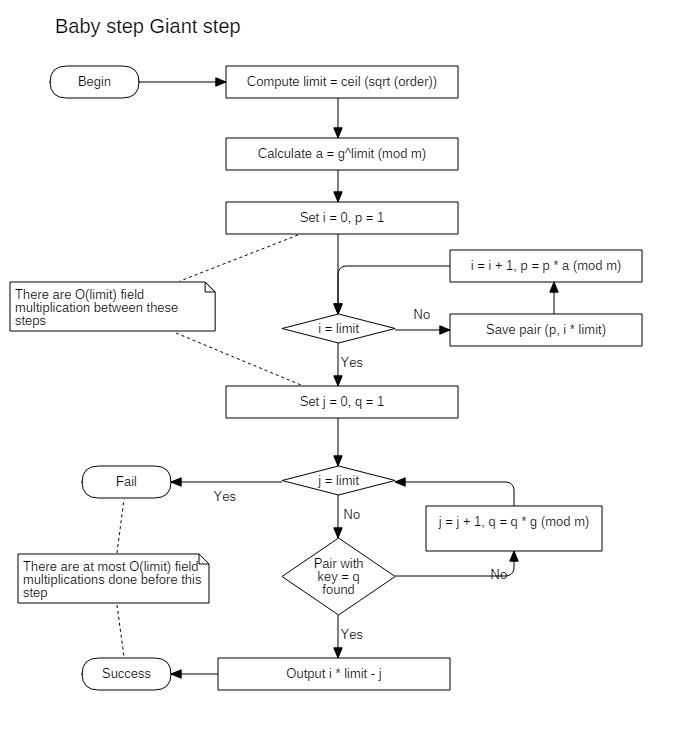
\includegraphics[scale=0.44]{bab2/img/bsgs}
	\caption{Diagram Alur Metode Penyelesaian Logaritma Diskret dengan \textit{Baby-step Giant-Step}}
	\label{fig:bsgs}
\end{figure}

Kompleksitas strategi ini bergantung pada metode pencarian di percabangan kedua ("\textit{pair with key = q found}"). Umumnya metode ini menggunakan metode pencarian \textit{binary search}. Konsekuensinya, penyimpanan pasangan \textit{(p, i * limit)} dilakukan secara terurut dan seluruh proses ini membutuhkan waktu $ O(\sqrt{n}\ log\ n) $. Kemudian dengan menggunakan \textit{binary search} pencarian dapat dilakukan dengan kompleksitas $ O(log\ n) $. Selain \textit{binary search}, dapat juga digunakan \textit{hash table} sebagai alternatif dimana pencarian dapat dilakukan selama $ O(1) $. Penggunaan salah satu dari kedua metode pencarian tersebut mengakibatkan kompleksitas metode \textit{Baby-step Giant-step} secara keseluruhan menjadi $ O(\sqrt{n}) $.

\subsection {Penjelasan Strategi Penyelesaian Logaritma Diskret dengan Baby-step Giant-step}

Persamaan \eqref{eq:persamaan_umum_pembagian} mendasari metode \textit{Baby-step Giant-step}, yaitu pembagian dua bilangan. Diberikan sebuah bilangan $ a $, apabila dibagi dengan sebuah bilangan tertentu $ x $, akan membentuk persamaan \eqref{eq:persamaan_dasar_bsgs}
\begin{equation}
a=qx+r
\label{eq:persamaan_dasar_bsgs}
\end{equation}

Pada persamaan \eqref{eq:persamaan_dasar_bsgs}, $ q $ berada pada rentang $ 0 \leq q \leq a $ dan $ r $ berada pada rentang 
$ 0 \leq r < x $. Umpamakan proses pencarian $ q $ dan $ r $ tidak dapat dilakukan dengan operasi pembagian dan mod. Pencarian nilai $ q $ dan $ r $ maka harus menggunakan pendekatan \textit{brute force}, yaitu mencoba semua kombinasi $ q $ dan $ r $ yang menyebabkan persamaan \eqref{eq:persamaan_dasar_bsgs} bernilai benar. Mengingat nilai $ q $ dan $ r $ bergantung pada nilai $ x $ yang digunakan, maka perlu dipilih sebuah nilai $ x $ yang menyebabkan daerah pencarian $ q $ dan $ r $ minimal. Variabel pada persamaan \eqref{eq:persamaan_dasar_bsgs} yaitu $ q $, $ x $, dan $ r $ memiliki hubungan satu sama lainnya. Hubungan ini dapat dilihat pada proporsi \eqref{eq:proporsi_var_persamaan_dasar_bsgs}.
\begin{equation}
\frac{1}{q} \propto x \propto r
\label{eq:proporsi_var_persamaan_dasar_bsgs}
\end{equation}

Variabel $ q $ dan $ x $ memiliki proporsi saling terbalik, yaitu apabila nilai $ q $ naik, nilai $ x $ akan turun. Kasus sebaliknya juga berlaku. Sedangkan variabel $ x $ dan $ r $ memiliki proporsi langsung, yaitu apabila nilai $ x $ naik, nilai $ r $ akan naik juga. Kasus sebaliknya juga berlaku. Untuk menghasilkan kombinasi $ q $ dan $ r $ yang minimal, nilai $ x $ harus dipilih supaya $ q $ dan $ r $ kurang lebih bernilai sama. Nilai $ x $ yang dapat digunakan adalah $ \sqrt{a} $, dimana $ q=\sqrt{a} $, dan $ x=r=\sqrt{a} $. Untuk menjamin $ \sqrt{a} \in \mathbb{Z}_n $, hasil $ \sqrt{a} $ dibulatkan ke atas. Persamaan \eqref{eq:persamaan_dasar_bsgs} kini dapat ditulis menjadi persamaan \eqref{eq:bsgs_dengan_akar_A}.
\begin{equation}
a=q\sqrt{a}+r
\label{eq:bsgs_dengan_akar_A}
\end{equation}
Sekarang, andaikata nilai $ a $ pada persamaan di atas merupakan nilai $ a $ yang sama pada persamaan logaritma diskret $ y \equiv g^a\ \Mod{n} $ (persamaan \eqref{eq:persamaan_umum_log_diskret}), persamaan di atas dapat diubah menjadi
\begin{align}
log_{g}\ y &= q\sqrt{a}+r \\
y &\equiv g^{q\sqrt{a}+r}\ \Mod{P} \\
y*g^{-r} &\equiv g^{q\sqrt{a}}\ \Mod{P}
\label{eq:bsgs_persamaan_utama_dengan_invers_r}
\end{align}
Maka apabila ditemukan nilai $ r $ dan $ q $ tertentu yang memenuhi bentuk persamaan \eqref{eq:bsgs_persamaan_utama}, logaritma diskret $ y $ dapat dihitung dengan menghitung $ q\sqrt{a}+r $. Sayangnya proses penghitungan $ q\sqrt{a}+r $ membutuhkan pencarian invers modulus $ g^r $, sebuah proses yang membutuhkan waktu komputasi yang cukup mahal. Hal ini dapat dihindari dengan sedikit mengubah persamaan \eqref{eq:bsgs_persamaan_utama}.
\begin{equation}
a=q\sqrt{a}-r
\label{eq:bsgs_dengan_invers_r}
\end{equation}
Dengan mengikuti proses transformasi persamaan \eqref{eq:bsgs_dengan_akar_A} menjadi persamaan \eqref{eq:bsgs_persamaan_utama_dengan_invers_r}, persamaan \eqref{eq:bsgs_dengan_invers_r} dapat diubah menjadi persamaan \eqref{eq:bsgs_persamaan_utama}.
\begin{align}
log_{g}\ y &= q\sqrt{a} - r \\
y &\equiv g^{q\sqrt{a} - r}\ \Mod{n} \\
y*g^r &\equiv g^{q\sqrt{a}}\ \Mod{n}
\label{eq:bsgs_persamaan_utama}
\end{align}
Dengan menggunakan persamaan \eqref{eq:bsgs_persamaan_utama}, logaritma diskret $ y $ dapat dicari tanpa harus mencari invers modulus $ g^r $. Yang perlu dilakukan sekarang adalah mencari pasangan $ r $ dan $ q $ yang memenuhi persamaaan \eqref{eq:bsgs_persamaan_utama}. Disinilah alasan metode ini disebut \textit{Baby-step Giant-step}. Pada sisi kiri persamaan \eqref{eq:bsgs_persamaan_utama}, nilai $ y*g^r $ dicari. Bagian ini merupakan \textit{baby-step} karena interval pangkat untuk basis $ g $ yang digunakan adalah $ 1 $ (nilai pangkat yang digunakan adalah $ \{0,1,2,\ldots,\allowbreak\sqrt{a}-1\} $). Bagian sisi kanan persamaan \eqref{eq:bsgs_persamaan_utama} disebut \textit{giant-step} karena untuk mencari nilai $ g^{q\sqrt{a}} $, interval pangkat untuk basis $ g $ yang digunakan adalah $ \sqrt{a} $ (nilai pangkat yang digunakan adalah $ \{0,\sqrt{a},2\sqrt{a},\ldots,(\sqrt{a}-1) \sqrt{a}\} $).
Persamaan \eqref{eq:bsgs_persamaan_utama_dengan_invers_r} dan persamaan \eqref{eq:bsgs_persamaan_utama} menyebabkan daerah pencarian $ r $ dan $ q $ turun menjadi $ O(\sqrt{a}) $.

\subsection{Strategi Penyelesaian Logaritma Diskret dengan Pollard Rho}
Metode \textit{Pollard Rho} awalnya adalah metode untuk melakukan faktorisasi bilangan \cite{brent_montecarlo}. Namun metode ini dapat dimodifikasi agar dapat digunakan untuk melakukan pencarian logaritma diskret.
Diberikan sebuah \textit{random function} $ f_n (x) $.
\begin{subequations}
	\[
		f_n (x)=
		\begin{cases}
		(\beta*x)\mod{n}, &\text{if } x\in S_1 \\
		(x*x)\mod{n}, &\text{if } x\in S_2 \\
		(\alpha*x)\mod{n}, &\text{if } x\in S_3
		\end{cases}
		\tag{\ref{eq:random_function}}
	\]
	\label{eq:random_function}
\end{subequations}
Terdapat tiga himpunan, $ S_1 $, $ S_2 $, dan $ S_3 $, masing-masing merupakan himpunan bagian $ \mathbb{Z} $, yang digunakan untuk menentukan persamaan $ f_n (x) $ yang digunakan. Tidak ada batasan yang terlalu mengikat dalam menentukan anggota ketiga himpunan ini selain ketiga himpunan ini harus memiliki kardinalitas yang kurang lebih sama, dan $ 1 \notin S_2 $.

Fungsi $ f_n (x) $ akan digunakan untuk proses \textit{step}. Proses ini dapat dijabarkan sebagai berikut.
\begin{enumerate}
\item Tentukan nilai $ f_n (x_0)=1 $
\item Cari nilai $ x_{i+1}=f_n (x_i) $
\end{enumerate}

Fungsi $ f_n (x) $ akan bekerja pada sistem modulus n (yaitu $ \mathbb{Z}_n^* $). Apabila proses \textit{step} dilakukan terus menerus, suatu saat akan ada nilai $ f_n (x_s) $ yang bernilai sama dengan $ f_n (x_t) $, $ s>t $. Hal ini disebabkan $ f_n (x) \in \mathbb{Z}_n $ , dan himpunan $ \mathbb{Z}_n $ memiliki jumlah anggota berhingga. Suatu saat keluaran fungsi $ f_n (x) $ telah merentang seluruh nilai $ \mathbb{Z}_n $ yang mungkin dibentuk, sehingga \textit{step-step} selanjutnya hanya mengulang permutasi nilai yang dihasilkan oleh $ f_n (x) $.\cite{brent_montecarlo}

Dengan diketahui dua nilai $ f_n (x_s) $ dan $ f_n (x_t) $, nilai logaritma diskret $ y $ dapat diketahui. Untuk itu, fungsi $ f_n (x) $ untuk suatu $ x $ perlu ditulis dengan persamaan \eqref{eq:persamaan_umum_step}.
\begin{equation}
f_n (x)\equiv \alpha^a \beta^b\ \Mod{n}
\label{eq:persamaan_umum_step}
\end{equation}

Kemudian jabarkan persamaan $ f_n (x_s)=f_n (x_t) $, $ s>t $ dalam bentuk persamaan \eqref{eq:persamaan_umum_step}.
\begin{align}
f_n (x_s) &\equiv f_n (x_t)\ \Mod{n} \\
\alpha^{a_s} * \beta^{b_s} &\equiv \alpha^{a_t} * \beta^{b_t}\ \Mod{n} \\
\alpha^{a_s-a_t} &\equiv \beta^{b_t-b_s}\ \Mod{n} \\
a_s - a_t &\equiv log_{\alpha} \beta * (b_t - b_s)\ (mod\ ord(\alpha))
\label{eq:persamaan_umum_step_logaritmik}
\end{align}
Dengan memasukkan nilai $ \alpha=g $ dan $ \beta=y $, persamaan \eqref{eq:persamaan_umum_step_logaritmik} memberikan nilai logaritma diskret $ y $.

Untuk menggunakan metode ini, dibutuhkan sebuah cara untuk mencari $ f_n (x_s) $ dan $ f_n (x_t) $ secara efisien. Subbab selanjutnya akan menjelaskan cara untuk menemukan $ f_n (x_s) $ dan $ f_n (x_t) $.

\subsection{Brent Cycle Detection}
Cara ini menggunakan dua buah \textit{pointer}, $ p_{\text{turtle}} $ dan $ p_{\text{hare}} $. Setiap proses \textit{step}, $ p_{\text{turtle}} $ melakukan 1 \textit{step}. Pointer $ p_{\text{hare}} $ bergerak setiap iterasi step ke $ 2^i $ dengan menyamakan posisinya dengan $ p_1 $. Gambar \ref{fig:brent_pollard_rho} menjabarkan metode ini secara detail.
\begin{figure}[h!]
	\Centering
	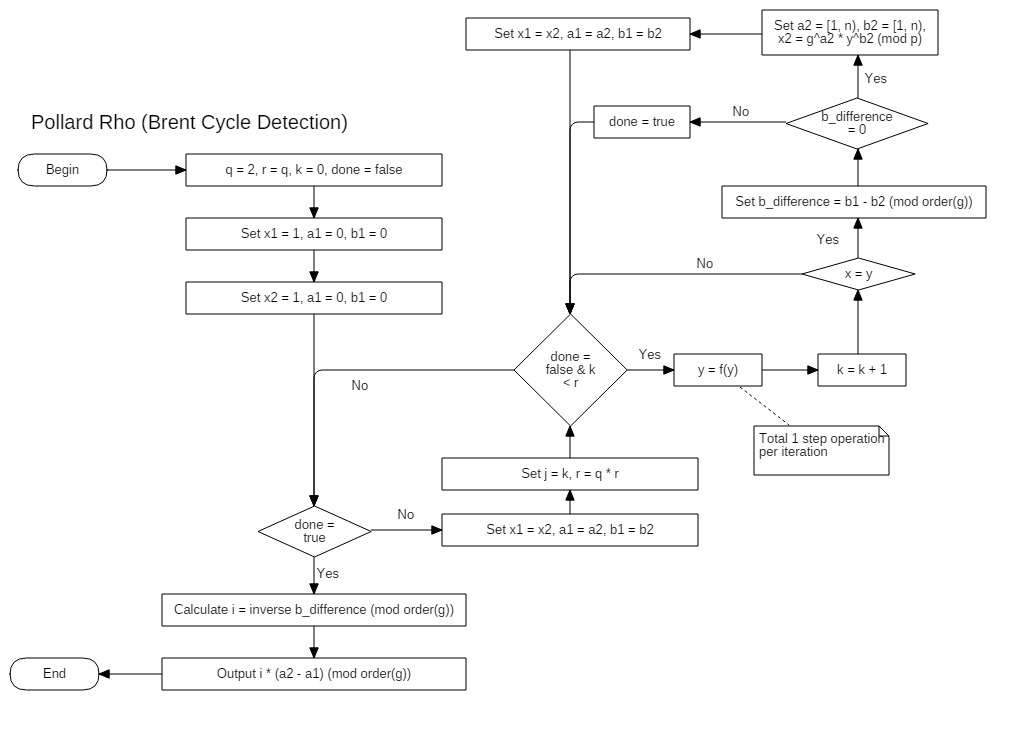
\includegraphics[scale=0.4,angle=90]{bab2/img/pollard-rho-brent}
	\caption {Diagram Alur Metode Deteksi Siklus Brent}
	\label{fig:brent_pollard_rho}
\end{figure}

Cara ini bisa gagal apabila selisih indeks pangkat $ \beta $ bernilai $ 0\ \Mod{n} $. Apabila hal tersebut terjadi, ulangi pencarian nilai $ p_{\text{turtle}} = p_{\text{hare}} $ dari awal, namun kedua \textit{pointer} dimulai dari $ f(x)=\alpha^i \beta^j\ \Mod{n} $, dimana $ 0 \leq i < n $ dan $ 0 \leq j < n $. \textit{Brent Cycle Detection} memiliki kompleksitas sebesar $ O(\sqrt{n}) $.

\section{Strategi Perkalian Modular}

Perkalian modular adalah persamaan \eqref{eq:persamaan_umum_perkalian_modular}.
\begin{equation}
a*b=c\ \Mod{n}
\label{eq:persamaan_umum_perkalian_modular}
\end{equation}

Sebelumnya telah dijelaskan bahwa terdapat kemungkinan terjadinya \textit{integer overflow} karena besarnya nilai $ p $. Maka perlu digunakan sebuah metode perkalian yang dapat menghindari kasus \textit{integer overflow}. Mengingat proses perkalian merupakan proses yang sering terjadi, metode tersebut juga sebaiknya memiliki kecepatan yang tinggi. Pada subbab ini akan dijabarkan dua metode perkalian yang dapat digunakan.

\subsection{Strategi Naif Perkalian Modular}

Strategi naif ini sebenarnya adalah persamaan \eqref{eq:mod_kali} yang ditulis dalam bentuk persamaan \eqref{eq:mod_kali_long}. Hal ini berguna untuk menekan nilai $ a $ dan $ b $ yang tinggi. Setelah dilakukan perkalian, terdapat kemungkinan hasil perkalian melebihi nilai modulus $ n $. Maka dari itu, hasil perkalian $ a $ dan $ b $ kembali dimodulus sekali lagi dengan $ n $. Gambar \ref{psdo:modmul_naive} memaparkan strategi yang dimaksud.

\begin{figure}[h!]
\begin{lstlisting}[firstnumber=0,captionpos=b]
NAIVE-MODULAR-MULTIPLICATION (a, b, n)
return ((a mod n) * (b mod n)) mod n
\end{lstlisting}
\caption{Pseudocode Metode Perkalian Modular Naif}
\label{psdo:modmul_naive}
\end{figure}

Metode ini dapat digunakan untuk $ n \leq 2^{32} $ karena hasil terbesar yang mungkin didapat dari perkalian modular dimana $ n \leq 2^{32} $ adalah $ a*b = c \Rightarrow ( 2^{32}-1 ) * ( 2^{32}-1 ) = 2^{64} - 2^{33} + 1 $. Nilai ini masih dapat ditampung menggunakan 64-bit \textit{integer}.

\subsection{Strategi Perkalian Modular dengan Logarithmic Modular Multiplication} 
Metode \textit{Logarithmic Modular Multiplication} merupakan analog dari \textit{Modular Expontiation} \cite{geeks_modular_multiplication}. Yang membedakan adalah ketimbang pemangkatan, \textit{Logarithmic Modular Multiplication} melakukan perkalian seperti yang ditunjukkan persamaan \eqref{eq:persamaan_umum_perkalian_modular}. Gambar \ref{fig:log_mod_mul} menjelaskan langkah metode ini.

\begin{figure}
	\Centering
	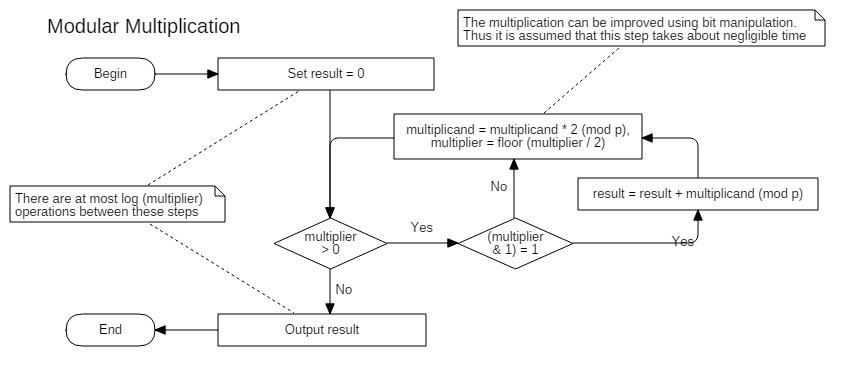
\includegraphics[angle=90,scale=0.5]{bab2/img/modular-multiplication}
	\caption{Diagram Alur \textit{Logarithmic Modular Multiplication}}
	\label{fig:log_mod_mul}
\end{figure}

Strategi ini memiliki kompleksitas $ O(log\ b) $.

\subsection{Penjelasan Strategi Perkalian Modular dengan Logarithmic Modular Multiplication}

Nilai $ b $ pada persamaan \eqref{eq:persamaan_umum_perkalian_modular} pertama-tama diubah menjadi sebuah polinomial \eqref{eq:dekomposisi_biner_perkalian}.
\begin{equation}
b=2^{0}*b_0+2^{1}*b_1+2^{2}*b_2+\ldots+2^{t}*b_t
\label{eq:dekomposisi_biner_perkalian}
\end{equation}
Kemudian kalikan kedua sisi persamaan dengan $ a $.
\begin{align}
ab &= a2^{0}*b_0+a2^{1}*b_1+\ldots+a2^{t}*b_t \\
ab &= \sum_{i=0}^{t} a2^{i}*b_i 
\label{eq:generalisasi_dekomposisi_biner_perkalian}
\end{align}
Maka perhitungan perkalian $ a $ dengan $ b $ merupakan persamaan \eqref{eq:generalisasi_dekomposisi_biner_perkalian}. Nilai $ a $ secara perlahan dikalikan dengan nilai $ 2^{i} $. Metode penghitungan persamaan \eqref{eq:generalisasi_dekomposisi_biner_perkalian} sama dengan cara penghitungan persamaan \eqref{eq:generalisasi_dekomposisi_biner_pemangkatan}. Apabila $ a_i = a * 2^i $, maka dengan memanfaatkan proses perkalian $ 2^i $ yang saling \textit{overlap} (seperti penghitungan $ 2^7 $ pasti membutuhkan hasil penghitungan $ 2^4 $) nilai $ a_i $ dapat ditulis dengan relasi \eqref{eq:relasi_rekurens_a_i}.
\begin{subequations}
	\[
	a_i=
	\begin{cases}
	a, 			& \text{if } i = 0 \\
	a_{i-1} * 2	& \text{if } i > 0
	\end{cases}
	\tag{\ref{eq:relasi_rekurens_a_i}}
	\]
	\label{eq:relasi_rekurens_a_i}
\end{subequations}
Kemudian diberikan sebuah nilai $ term(x)=a_x * b_x $. Maka $ term(x) $ dapat ditulis menjadi persamaan \eqref{eq:relasi_termx}.
\begin{subequations}
\[
	term(x)=
	\begin{cases}
		0, 		& \text{if } b_x=0 \\
		a_i		& \text{if } b_x=1
	\end{cases}
	\tag{\ref{eq:relasi_termx}}
\]
\label{eq:relasi_termx}
\end{subequations}
Sehingga persamaan \eqref{eq:generalisasi_dekomposisi_biner_perkalian} dapat ditulis menjadi persamaan \eqref{eq:generalisasi_dekomposisi_biner_perkalian_rekursif}.
\begin{equation}
	ab = \sum_{i=0}^{t} term(i)
	\label{eq:generalisasi_dekomposisi_biner_perkalian_rekursif}
\end{equation}

Untuk menghitung nilai $ a_i $, kalikan nilai $ a_{i-1} $ yang tersimpan dengan 2. Cara ini dapat digunakan hingga $ a_{(\log b)} $ sehingga penghitungan $ f(n) $ akan membutuhkan $ O(\log b) $ proses perkalian dengan dua. Konsekuensinya, persamaan \eqref{eq:relasi_termx} membutuhkan $ O(\allowbreak\log b) $ proses perkalian. Metode ini dapat digunakan untuk perkalian hingga 63-bit.

\section{Landasan Terkait Pengujian Kebenaran Program}
Keluaran program yang akan digunakan untuk menyelesaikan permasalahan perlu diujikan kebenarannya. Untuk itu perlu dibuat masukan yang mengikuti penjelasan soal seperti yang telah diterangkan pada subbab \ref{sec:Parameter Masukan}. Beberapa teori dan landasan yang akan dimanfaatkan untuk membuat parameter masukan akan dijabarkan pada subbab ini.

\subsection{Miller-Rabin Primality Test}

Subbab ini menjelaskan sebuah metode untuk melakukan pengecekan keprimaan sebuah bilangan, yaitu \textit{Miller-Rabin Primality Test}. Metode ini akan digunakan untuk membangun beberapa parameter.

Metode pengecekan keprimaan \textit{Miller-Rabin} digunakan sebagai alternatif metode pengecekan keprimaan secara naif (dimana metode tersebut memiliki kompleksitas $ O(\sqrt{n})) $. Metode ini menggunakan dasar bahwa apabila terdapat sebuah bilangan ganjil $ n $, kemudian dicari nilai $ s $ dan $ r $ yang memenuhi persamaan $ n-1=2^{s} r $, dan apabila $ n $ merupakan bilangan prima, maka setidaknya salah satu dari kedua persamaan berikut akan bernilai benar. \cite{hac_publickey, stallings_cryptography}
\begin{align}
\label{eq:miller_rabin_condition_1}
a^r &\equiv 1\ \Mod{n}, & \gcd(a,n)=1 \\
\label{eq:miller_rabin_condition_2}
a^{2^j r} &\equiv -1\ \Mod{n}, & \gcd(a,n)=1,\ 0 \leq j <s-1
\end{align}
Persamaan \eqref{eq:miller_rabin_condition_1} dan \eqref{eq:miller_rabin_condition_2} memberi batasan tersirat $ a>0 $. Untuk seterusnya, nilai $ a $ akan diasumsikan jatuh pada rentang $ 1 \leq a < n $.

Untuk $ n $ yang berupa bilangan prima, salah satu dari persamaan di atas pasti akan terpenuhi. Namun untuk $ n $ yang bukan merupakan bilangan prima, terdapat nilai $ a $ yang memenuhi kedua persamaan di atas. Bilangan $ a $ ini umum disebut dengan \textit{strong liar} terhadap keprimaan $ n $. Artinya, bilangan $ a $ seolah-olah menunjukkan bahwa nilai $ n $ merupakan bilangan prima sebab nilai $ a $ tersebut memenuhi persamaan \eqref{eq:miller_rabin_condition_1} atau \eqref{eq:miller_rabin_condition_2}. Kehadiran \textit{strong liar} untuk $ n $ paling banyak berjumlah $ \frac{1}{4} \phi(n) $ dimana $ \phi(n) $ merupakan \textit{Euler Totient Function}. Artinya kemungkinan nilai komposit $ n $ dianggap sebagai bilangan prima paling besar adalah $ 25\% $. \cite{hac_publickey}

Kemungkinan terjadinya galat pada metode \textit{Miller-Rabin} dapat diperkecil dengan beberapa kali mengecek nilai $ a $ yang berbeda-beda. Untuk $ t $ kali percobaan, kemungkinan terjadinya galat pada metode \textit{Miller-Rabin} adalah paling banyak $ (\frac{1}{4})^{t} $. Semakin besar nilai $ t $, semakin kecil kemungkinan terjadinya galat. \cite{hac_publickey}

\textit{Miller-Rabin} awalnya adalah metode probabilistik untuk menentukan keprimaan sebuah bilangan. Namun dengan membatasi nilai yang akan diperiksa jatuh pada rentang $ 2 \leq n < 2^{64} $, metode \textit{Miller-Rabin} berubah menjadi metode deterministik. Online Encyclopedia of Integer Sequence \cite{oeis_mrabin_limit} menjabarkan sederet nilai yang merupakan nilai batas atas pengujian Miller-Rabin yang tidak akan menghasilkan keluaran yang salah jika diujikan dengan himpunan nilai $ a $ tertentu. Himpunan ini merupakan $ i $ bilangan prima pertama dimana $ i $ adalah suku ke-i pada deretan nilai batas atas. Tabel \ref{tab:miller_rabin_deterministic_a} berisi himpunan yang dimaksud.

\begin{table}[h!]
	\caption{Himpunan Bilangan Pengecek Keprimaan Miller Rabin Jika N Kurang Dari Batas Atas}
	\label{tab:miller_rabin_deterministic_a}
	\ttfamily
	\begin{tabularx}{\linewidth}{ |l|l|X| }
		\hline
		i&	Batas Atas&	\{a\} \\
		\hline
		1&	2047&	2 \\
		2&	1373653&	2, 3 \\
		3&	25326001&	2, 3, 5 \\
		4&	3215031751&	2, 3, 5, 7 \\
		5&	2152302898747&	2, 3, 5, 7, 11 \\
		6&	3474749660383&	2, 3, 5, 7, 11, 13 \\
		7&	341550071728321&	2, 3, 5, 7, 11, 13, 17 \\
		8&	341550071728321&	2, 3, 5, 7, 11, 13, 17, 19 \\
		9&	3825123056546413051&	2, 3, 5, 7, 11, 13, 17, 19, 23 \\
		10&	3825123056546413051&	2, 3, 5, 7, 11, 13, 17, 19, 23, 29 \\
		11&	3825123056546413051&	2, 3, 5, 7, 11, 13, 17, 19, 23, 29, 31 \\
		12&	318665857834031151167461&	2, 3, 5, 7, 11, 13, 17, 19, 23, 29, 31, 37 \\
		\hline
	\end{tabularx}
\end{table}

\subsection{Polinomial Pembuat Bilangan Prima}

Pencarian bilangan prima dapat dilakukan dengan mencoba nilai satu per satu dan mengecek apakah nilai tersebut merupakan bilangan prima atau bukan. Cara ini cenderung tidak efektif. Untuk mempersingkat waktu pencarian bilangan prima, digunakan sebuah polinomial penghasil prima.

Polinomial pembuat bilangan prima yang digunakan adalah polinomial \eqref{eq:polinomial_pembuat_prima}. \cite{wolfram_prime_polynomial}
\begin{equation}
f(n)=n^2+n+41
\label{eq:polinomial_pembuat_prima}
\end{equation}

Walaupun polinomial \eqref{eq:polinomial_pembuat_prima} disebut dengan polinomial penghasil prima, keluaran polinomial ini belum tentu selalu bilangan prima sehingga perlu dilakukan pengecekan keprimaan. Kendati begitu, penggunaan polinomial ini mampu mempercepat pencarian bilangan prima dibandingkan metode naif.
